\chapter{{Speech communities}}

This is the second of two chapters with a focus on socio-historical data that respond to research questions about the sailors and their speech communities. This chapter on the speech communities specifically attempts to characterize the immediate and extended contexts in which sailors were likely to work and socialize. The data presented support the claim that the speech communities of English-speaking sailors were extensive and robust enough to develop distinct features of speech likely to have been recognized by those outside the community as a distinct sailors’ variety. The data also speak to how \isi{language transfer} and change may have been affected by the social networks that bound these communities and maintained their distinct language variety. The chapter is presented in two sections. Firstly, the section on Insular Ship Communities presents data on sailors’ duration at sea, autonomy and violence, social order and disorder, subgroups and \isi{social cohesion}, the role of alcohol, and shared ideologies and leisure activities. The second section dealing with Wider Maritime Communities presents data on profuse maritime activity, convoys and communication, the \isi{maritime economy}, corruption and theft, sailors on land, and contact with port communities. 

\section{{General considerations}}\label{sec:4.1}

The fact that most linguists have neglected to address the nature or importance of \isi{maritime speech} communities is perhaps not surprising. Not only do these speech communities fail to fit into a traditionally defined geographical region or single social stratum, but their composition has also been obscured by centuries of non-existent, falsified, and fragmentary record-keeping. Even in the context of managing the records of a single nation’s trade activity and using only one language, records are often woefully inadequate to reflect the real nature of trade and communication, e.g., \citeauthor{Cook2005}’s investigation into \isi{seventeenth century} litigation against a captain in the English coastal shipping trade indicates, “\textit{almost one third} of the working runs escaped the official records in the normal pattern of trading” (2005: 15, emphasis added). Even in consideration of specific ports, record-keeping was typically unofficial and subject to private publication. For example, London shipping was unofficially reported in local pamphlets like the \textit{Lloyd's List} (first published c. 1764) circulated among clients of the Lloyd’s coffee house that served as a center of maritime information and insurance. These lists contained selected commercial information and details of vessels arriving at ports in England and Ireland, and it was not until 1760 that the underwriters who frequented Lloyd’s of London combined to form an association with the aim of producing a more complete Register Book of Shipping, circulated since 1734\footnote{Merseyside Maritime Museum Archives \& Library. (2010).  \textit{Lloyds Marine Insurance Records} (Information Sheet: 52). Retrieved from \url{http://www.liverpoolmuseums.org.uk/maritime/archive/sheet/52}}. Likewise, although \isi{Liverpool}’s shipping was subject to a series of Acts of Parliament requiring that details of vessels be registered, such record-keeping was haphazard up until the Registry Act of 1786\footnote{Merseyside Maritime Museum Archives \& Library. (2010).  \textit{\isi{Liverpool} Ship Registers} (Information Sheet: 50). Retrieved from \url{http://www.liverpoolmuseums.org.uk/maritime/archive/sheet/50}}. Thus, the sources of information on shipping movements and \isi{crew} composition that might inform research on \isi{maritime speech} communities, if they existed at all before 1750, were localized, selective, privately published, and almost invariably lost to the archival record. 

The problem of insufficient data is magnified exponentially in the context of inconsistent record-keeping in \isi{transatlantic} commerce that was conducted in various languages and ranged across multiple ports operated by different European nations on four continents. Jarvis’ detailed study of Bermudan maritime activity concludes “London missed much of what happened in the colony” (\citealt{Jarvis2010}: 461). And this could be said of most of the colonies of the time, given that imperial record keeping primarily targeted large bulk shipments of goods and is silent on the abundant maritime activity in local trade and the logging, salvage, turtling, and salt-raking trades of the Atlantic commons that sailors actively concealed from the Board of Trade’s custom officials. As a result, Jarvis claims that “much of the North American coast and virtually the entire Caribbean had permeable and blurry maritime borders” (\citealt{Jarvis2010}: 462). In addition to these blurry areas of imperial oversight, even when records were kept, there was often little verification of their accuracy, for example, one letter from a Virginia court trial details how easy it was to evade port charges with falsification of docking registers, “they give her [the ship] the name of the \textit{Alexander}... at other times they will change her name, and call her the \textit{providente-galley}” [CO 5/1411/631]. In short, I acknowledge that empirical data is limited on this subject.  Therefore, the following sections on the common characteristics of maritime communities are based largely on qualitative data, in an attempt to characterize the real communities that were often absent from the quantifiable data of the official records.

\section{{Insular ship communities}}\label{sec:4.2}

Working aboard an early colonial vessel was no day job; sailors lived at sea and the vessels they lived on were comparable to small towns. One passenger on a \isi{voyage} from Europe to Africa in 1666 notes in his journal: 

\begin{quotation}
The ship was like \textit{Noah’s} ark, for there were aboard it so many several sorts of beasts, that what with the noise, and the talk of so many people as were aboard, we could not hear one another speak… [the ship] looked like a castle on the sea [445f.1/509.]
\end{quotation}

It was common for men to “run away to sea” \citep[67,]{Jarvis2010} the very expression suggesting that the vessel was primarily a destination rather than a means of transportation. Similarly, in a letter dated 30 July {1699}, “they would not liarn [learn] from whense they came, nor whither they were bound, for they all told him yet his way \textit{bound to sea}” [CO 5/1411/631, emphasis added]. Indeed, the wooden sea-going vessels of the early \isi{colonial period} were communities in every sense of the word which could be just as large and complex as on land, e.g., one ship’s captain complained that “I was informed there was a surgeon belonging to the ship but never saw him till I returned from Newcastle” (cited in \citealt{Brown2011}: 48) stressing the large nature of the ship and its sizable population. These floating communities, just like those on land, had their own rituals of social identity and order in addition to language practices that were unique to their context.

\subsection{{Duration at sea}}\label{sec:4.2.1}

The time that workers were expected to remain in a vessel was a key determining factor in the formation of a sea-going community identity. When sailors could no longer return home after a day at sea or a week’s short trading journey around local coasts, the notion of what their “home” was may have radically shifted from a port-based traditional notion of house and family to the assigned quarters or hammock and mess mates of their vessels. As trade and naval operations extended across the Atlantic, and particularly after the English involvement in the \isi{slave trade} increased after the Royal Charter of 1562, more sailors found themselves serving on \isi{transatlantic} journeys, described as “an ocean \isi{voyage} that could last from five weeks to three months” (\citealt{Brown2011}: 107). So, even if a ship sailed directly to a single port across the Atlantic, then spent minimal time managing cargo and sailed directly back to the same home port, the journey would still take an average of two to six months. However, the reality of shipping practice meant that sailors were likely to be away from land much longer than this. Even small sloops that might be expected to return to home port more frequently than larger vessels did not necessarily do so, but instead, as \citeauthor{Jarvis2010} explains, “made several round trips between North America and the Caribbean during the summer and fall seasons before returning home” (2010: 111).  He goes on to say that although small vessels did not typically make one \isi{transatlantic} \isi{voyage} per year as the larger ships did, they nonetheless were at sea for long durations as they made multiple short voyages “at least two or three and in some cases as many as fourteen round-trips in a single year” (\citealt{Jarvis2010}: 125). The common practice of stopping in multiple ports on circum-Atlantic journeys rather than travelling to a single destination and back again increased time at sea, and this was not only for reasons of legitimate trade but was also necessary for collecting food provisions, wood and water and enabling enterprising captains to take advantage of international entrepôts of trade which evaded harsh duties on export and import goods. In addition, the circum-Atlantic pattern of trade winds favored sailing vessels that set circular navigational courses (see \figref{fig:key:4.1}) 


\begin{figure}
\caption{\label{fig:key:4.1} The Atlantic Trade Winds in January and July. Adapted from Encyclopaedia Britannica.
%
Such circular navigation developed the trade system of taking manufactured goods out of Europe; collecting spices, gold and slaves in African ports, bartering for flour, meat and lumber in the Americas and Caribbean, and bringing cotton, fur, lumber and tobacco back to Europe on the return leg. Such circum-Atlantic trade routes are evidenced in  {seventeenth century} records, for example, one  {sailor}’s account of his international movements:
}
 

% \includegraphics[width=\textwidth]{figures/delgado-img8.gif}
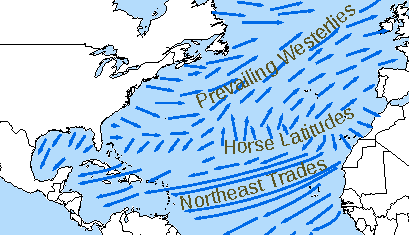
\includegraphics[width=\textwidth]{figures/atlantic.pdf}
\end{figure}


\begin{quotation}
[the \isi{deponent}] sailed from England being bound for \isi{Jamaica}, and arrived at \isi{Jamaica} in may following… and stayed in \isi{Jamaica} about a month…[then.].. he made a tripp over to new Yorke, where he staied two months or thereabouts...he sailed again with the said shipp to \isi{Jamaica} ...he sett saile from \isi{Jamaica} being full laden with sugar cottons and other wares… but in his passage to London he mett with foule weather and lost his foremast and threby was forced to putt into Boston in new England where he arrived on or about ….August last past and staid there until he had fitted the said ship, which being done he sailed from Boston ...for London, but in his passage he lost his rudder was forced into...the West of England [HCA 1/52/20.]\end{quotation}

Journeys such as the one described above that navigated around extended trade networks were invariably prolonged by inconstant weather and storms as well as by the time required for  checking, loading and unloading cargo and provisioning and maintaining the ship, and thus required crews to spend significantly more than a few months aboard the vessel. 

It is possible to calculate a rough average of the average \isi{sailor}’s duration at sea, although doing so necessarily obscures the differences between the types of vessels, types of voyages, and ranks of the \isi{crew} that likely created very different profiles for different groups of people. Yet, with this caveat in mind, 53 first-hand records in which sailors refer to their individual duration at sea, based on witness testimony in court records and comments in private letters and journals, the average time at sea was 15.73 months, or one year, three months and 23 days (see \figref{fig:key:4.2}) This average duration that individuals reported at sea is corroborated by the data in 84 logbooks that generate an average \isi{voyage} duration of 14.46 months, or one year, four months and 14 days (see \figref{fig:key:4.3}) Furthermore, these two sets of data also align with data cited in secondary sources, such as the comment describing the duration at sea for the \isi{crew} of the \isi{late sixteenth century} ship \textit{Harve,} “They had been gone for over fourteen months” (\citealt{Bicheno2012}: 124). Hence, the triangulated data suggests that a typical \isi{sailor} in the \isi{transatlantic} trade could expect to spend at least one year and a quarter continuously serving at sea at any one time. 

However, we should not suppose that after a \isi{voyage} of over a year, sailors returned to their homes on land. Compelling evidence suggests that many sailors signed on for (or were forced into) consecutive voyages that might have taken them away from life on land indefinitely. For example, many of the data composing \figref{fig:key:4.2} about individual durations at sea come from court trials of sailors accused of piracy who merely state how long they had been serving on the vessel from which they were arrested, e.g., “has been about 18 mos with the Rogues” [HCA 1/99/135] and another \isi{sailor} who was “taken...19 months ago [and.].. had not had any Opportunity Since of Escaping” [HCA 1/99/105.]


\begin{figure}
%%[Warning: Draw object ignored]
%%[Warning: Draw object ignored]
  

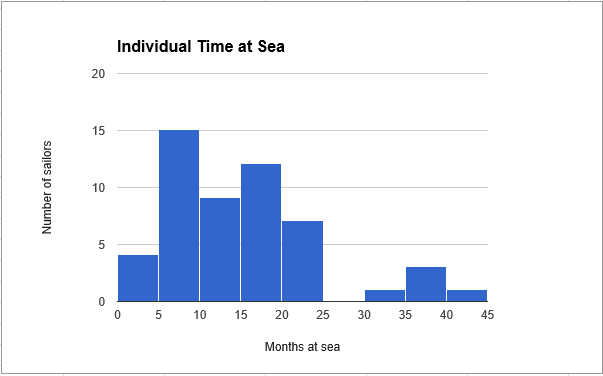
\includegraphics[width=\textwidth]{figures/delgado-img9.png}
 

\caption{\label{fig:key:4.2} Individual time at sea based on witness depositions, letters and journals\textsuperscript{a} }

\textsuperscript{a} Sources: 445f.1/485,486; DDB6 8/4; HCA 1/101/124; HCA 1/13/96; HCA 1/14/17,19; HCA 1/52/20; HCA 1/52/48; HCA 1/9/63; HCA 1/98/252,259,56,57,9; HCA 1/99/102; HCA 1/99/104,105,109,114,116,117,120,121,125,127,128,130,131,132,133,135,140,146,150,155,157,159,162,165,167,170,72,73,80,86,88,89,90,93,94
\end{figure}


\begin{figure}
%%[Warning: Draw object ignored]
%%[Warning: Draw object ignored]
  

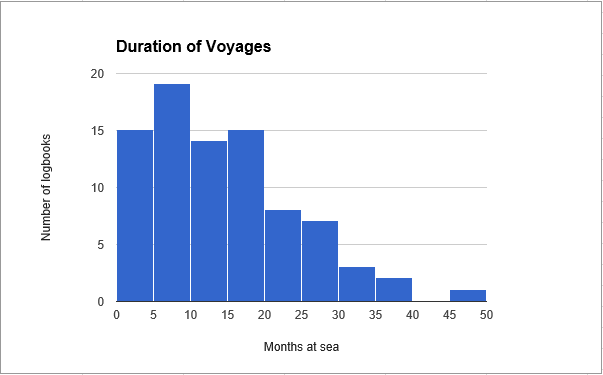
\includegraphics[width=\textwidth]{figures/delgado-img10.png}
 

\caption{\label{fig:key:4.3} Duration of voyages based on ships’ logbooks\textsuperscript{a}}

\textsuperscript{a} Sources: ADM 52/1/11; ADM 52/2/1-9; ADM 52/3/1-13; ADM 51/4322/1-6; ADM 51/3983/1-4; ADM 51/3954; ADM 51/3946/1-6; ADM 51/3946/1-13; ADM 51/4170/1-10; ADM 51/3797/1-8; T/70/1215
\end{figure}


Thus, it is likely that these individuals had served at sea for longer than their stated duration because this only reflects the time spent with the \isi{crew} of the most recent vessel they were on. Additionally, and as previously discussed in \sectref{sec:3.2} low-ranking sailors were routinely “turned over” from one vessel to another before reaching home ports. This practice kept men at sea for much longer periods of time that the actual sailing routes or military postings lasted (\citealt{AdkinsAdkins2008}: 365). For example, John Stretton describes consecutive voyages starting with his employment at New York for a \isi{voyage} to Virginia, and then after to England, Holland, New York again and Philadelphia Bay before terminating his term of service in Hamburg [HCA 1/14/140]. Likewise, another \isi{sailor} is appointed in New York and sails to \isi{Jamaica}, Lisbon and back again to New York before heading off to Antigua and then again to North America, including ports on the St. Lawrence river [HCA 1/98/15]. 

Furthermore, many of the lowest-ranking sailors were denied shore leave for fear of desertion. Sailor testimonies describing the strict enforcement of this rule range from statements attesting to how one ship’s master “would not suffer me to go on Shore” [HCA 1/99/5] to the consequences of breaking such mandates, as when the “Master went to the mate and gave him a blow on the face with his fist asking him what he did ashoare” [HCA 1/52/45]. So, it appears not to have been uncommon for sailors to be at sea for years without enjoying shore leave, let alone returning to the home port they had disembarked from. Indeed, the situation was often so repressive that some sailors chose to risk death in the water or upon unknown shores rather than stay aboard any longer, e.g. in the 1700 trial of John Houghling, Corneluis Franc and Francois Delaune, one witness testifies “I saw three or four jump into the water expecting they would make towd the shore I wan to meet them but only one came [ashore]” [CO 5/1411/39]. Additionally, the fact that sailors were so rarely on land caused problems for the courts, e.g. the petition of David Creagh in 1675 claims that he knows many men who might be able to testify to his innocence, “but being seafareing men he cannot hope to find them always on shore, nor to have the benefitt of their Testimony...they being bound for sea” [HCA 1/13/104] and also the complaint of a plaintiff who was awarded restitution from one \isi{sailor}, but laments “he believed he shou’d never come to England to pay it”  [HCA 1/99/97]. In short, although \isi{transatlantic} trips could be theoretically made in a few months, it was more likely that voyages took more than a year and additionally likely that sailors served on consecutive voyages, potentially without shore leave, thus creating alternative and relatively stable societies at sea that may have been periodically re-populated, but were invariably composed of workers who spent the greater part of their lives off shore. 

\subsection{{Autonomy and violence}}\label{sec:4.2.2}

Many of the floating communities operating in the murky waters of early colonial trade were largely autonomous as a result of the inability of imperial Britain to effectively regulate them and the existence of international networks of \isi{contraband} trade and communications that enabled them to operate on the captain’s authority. Indeed, a captain might appeal to the men to recognize his own authority regardless of British law, as if the insular communities of the sea were somehow self-regulating and therefore subject only to internal justice and authority. For example, in the \isi{late sixteenth century}, Francis \isi{Drake} appealed to the \isi{crew} “My masters, you must judge for yourselves whether or not this fellow has tried to undermine my authority… let they who think this man deserves to die hold up their hands” (cited in \citealt{Bicheno2012}: 140). The type of power that captains like \isi{Drake} asserted created a pseudo-democratic microcosm of the contemporary British nation-state aboard ship\footnote{\isi{Drake} is described as “pseudo-democratic” because even in his seemingly democratic appeal to his \isi{crew}, the men he addressed knew their expected complicity in the execution of Thomas Doughty and how unwise it would have been to speak against the wishes of the aggressive and assertive young officer poised to take command.}  and this system of government was what enabled insular communities of pirates, freebooters and buccaneers to manage and regulate social order in societies that were marginalized even within the maritime world. The benefits of such insular autonomy were twofold: firstly, it enabled captains to do as they pleased without concern for home legislation, and secondly, it offered the British government a degree of plausible deniability when such captains were engaged in international raiding against supposed trading allies or in nefarious activities that were in the government’s interest but which it could not openly support. For example, William Wilkinson, \isi{mariner} of London, explains how English Captains working for the African Company were allegedly sent to seize \isi{merchant} ships and cargos regardless of nationality: 

\begin{quotation}
other Commanders have had a share of the Ships and Cargo’s that have been so illegally seized… and their business has been to destroy and devour the Ships and Estates of English Subjects, and share them as their own… who ought to protect their Merchants Ships in trade [BL/74/816/m/11/36/3]. 
\end{quotation}

\citeauthor{Fusaro2015} explains how some captains abused the concept of an onboard democracy owing to the fact that many co-owned the vessels they governed (2015: 23). This emboldened many commanding officers to assert feudal authority over what they considered to be their property (including the workers) with a type of coercion that Ogborn describes as “state-sanctioned violence exported from England” (cited in \citealt{Fury2015}: 4--5). Furthermore, such appropriation of absolute power often went unchecked by courts in Britain whose judges were politicians rather than defenders of the law. \citeauthor{Fusaro2015} explains that the priority of the courts at the time was to protect trade, and therefore “sentencing was not necessarily in line with strictly operational, or literal, interpretation of existing laws and customs” (2015: 23). Free traders, whether they operated strictly within the existing British laws or not, were often given the freedom of the seas and their superficial acknowledgement of legal processes, custom and duties is well represented in the contemporary description of how such private trading vessels would operate “looking one way and rowing another” [BL/J/8223/e/4/27/3]. Captains’ disdain of trading regulations frequently prompted response from colonial territories, e.g., a joint petition to British administrators written in {August 1709} by proprietors of \isi{Barbados} bemoans “the Liberty given to Separate Traders; which, unless remedied in time, is like to prove fatal, not only to us, but to the \textit{British} Trade upon the aforesaid Coast” [BL/J/8223/e/4/27]. In such a context, captains’ abuses of power over their poorest workers was a minor concern, particularly as such people were perceived as worthless and idle by their home government anyway. 

Tyrannical captains and superior officers, although of little concern to home authorities, were the target of regular complaint by sailors. Abuses of power were so common that even some in authority recognized the dangers of power imbalances, e.g., Captain Samuel Burgess writes “I was never known to be Shart or Severe with any Mann tho I had the advantage soe to bee” [HCA 1/98/57], and Samuel Pepys, in his diary of 1666, comments that pilots “dare not do nor go but as the Captains will have them; and, if they offer to do otherwize, the Captains swear they will run them through” (cited in \citealt{Lavery2009}: 75). However, based on the profusion of depositions detailing abuses of power by those in command, we can assume that the concerns of those such as Burgess and Pepys were outweighed by the desires for power that persuaded others to perpetuate the status quo. Some of the recoverable grievances brought to court included mild complaints of “ill usage” [SP 89/25/229], “garrulous language” [ADM 52/1/8], and “being continually abused by an Idle master who was drunk every day” [E134/34Chas2/Mich36], yet more commonly, sailors presented complaints of physical threats from superior officers, e.g., threats to cut a \isi{sailor}’s ears off for lack of compliance with orders [HCA 1/99/24; HCA 1/99/98], one Quartermaster’s threat to throw a \isi{sailor} overboard for waking him when he should have been on duty [HCA 1/52/124], and another \isi{sailor}’s concern that because of “the ill Usage of Capt. Williams... [he] was in continual Fear of his Life” [HCA 1/99.618]. Furthermore, evidence indicates that these were not idle threats. \tabref{tab:key:4.1} below provides excerpts from ten testimonies evidencing \isi{physical violence} and \tabref{tab:key:4.2} below provides excerpts from eleven testimonies evidencing \isi{physical violence} that resulted in the death of the victim.

\begin{table}
\caption{\label{tab:key:4.1} Samples of court testimony detailing physical abuse from superior officers}

\begin{tabularx}{\textwidth}{lQl}
\lsptoprule

\textbf{Complaint} & \textbf{Details} \textbf{of} \textbf{physical} \textbf{abuse} & \textbf{Source}\\
\midrule
Torture, Imprisonment & “clapt upon his leggs abt 8 or 9 pound weight...put into the stocks, where he lay 37 houres and after he had indured imprisonment for 46 days” & HCA 1/52/47\\
Violence & “their Captain...beat them Severely when they Disobeyed” & HCA 1/99/10\\
Violence & “The Quarter Master of the Pyrates beat him and forced him in again” & HCA 1/99/18\\
Violence & “it was out of his power to deny without hazard of beating” & HCA 1/99/31\\
Violence & “he was beat very much ... denying their Order” & HCA 1/99/32\\
Violence & The Boatswain “beat the Crew, for not being brisk enough” & HCA 1/99/41\\
Severe beating & “gave him more blowes and kicked him...blowes around the head, till the blood ran down from his nose and face” & HCA 1/52/22\\
Severe beating & “Comander fell on him and beate him very violently with his Cane” & HCA 1/52/127\\
Severe beating & “his head broke, and a hearty drubbing... Several Months unable for Duty” & HCA 1/99/72\\
Severe beating & “very sick with severall wounds the captain had given him on the back” & HCA 1/14/201\\
\lspbottomrule
\end{tabularx}
\end{table}


\begin{table}
\caption{\label{tab:key:4.2} Samples of court testimony detailing physical abuse from superior officers that resulted in death}
 
\begin{tabularx}{\textwidth}{p{3cm}Ql}
\lsptoprule

\textbf{Complaint} & \textbf{Details} \textbf{of} \textbf{physical} \textbf{abuse} \textbf{resulting} \textbf{in} \textbf{death} & \textbf{Source}\\
\midrule
Cruelty leading to suicide & “the said George Rowe did soe Barbarously \& Cruelly use [him.].. throwing himselfe...into the Sea to avoyde his Masters Cruelty” & HCA 1/11/110\\
Beaten to death & “ beat him..., and with his foote or knees or both stampt upon him and bruised his stomach with such violence... soon after dyed” & HCA 1/11/111\\
Beaten to death & Lieutenant George Bing, stands trial for beating a \isi{sailor} under his care to death with “a Cane” [Acquitted] & HCA 1/12/111\\
Beaten to death & “beate him and threw him downe headlong on the Quarter Deck upon which the said Robert Day fell sick and dyed about three weekes after” & HCA 1/52/127\\
Beaten to death & John Rogers received blows from his Captain, allegedly causing death & HCA 1/52/41\\
Beaten to death & John nightingall, a great many blows on the Head, very black \& blew & HCA 1/52/148\\
Beaten to death & “[the captain] took a cane of  moderate size...and gave the Deceased two or three Blows about the Head and Shoulders” [Acquitted] & HCA 1/99/8\\
Beaten to death & John Morris beaten “severall times very violently... he struck all of his teeth out of his head... laid for about 5 weeks and then died” [Guilty] & HCA 1/52/48\\
Beaten to death & “many bruises...his being beaten might be the occasion of his death” & HCA 1/52/176\\
Executed & “the Prisoner with two more [men] were sentenced to Death for attempting an Escape from them, and that the other two were really Shot for it” & HCA 1/99/50\\
Executed & “Were for deserting sentenced to Death over a Bowl of Punch” & HCA 1/99/125\\
\lspbottomrule
\end{tabularx}
\end{table}

Furthermore, when complaints were made, sailors’ concerns were dismissed outright, as one \isi{seaman} found out when he took his complaint of being beaten by the ship’s carpenter to the captain, who “called him a Drunken Rogue and bid him be gone to his Hamock” [HCA 1/52/22]. Others who tried to voice their concerns in court were similarly silenced, such as the \isi{sailor} who complained by letter that there was too little value placed on common sailors’ lives and was hauled before high court to explain himself, publicly retract his complaint, and apologize [HCA 1/99 Philadelphia, Oct 15 1731, 9--10]. Another \isi{sailor} finds so little justice that his last act of life after receiving a mortal beating from the ship’s chief mate is to write a letter of testimony to the only person likely to care:

\begin{quotation}
Ever Loufing wief these lines is to arkquint you that I Lying more like to die than to lief desiring you to remember my kind love to my three Cussons: and so Lying in this condission throw the means of the Cheaf mat of the Ship Bengdall marchant: Rodger Nubery be knowd: so I Laying my Death to the Sadd Rodger Nubery: hear I seal my John Morris [HCA 1/52/51]. \end{quotation}

It is worth noting that all the testimony presented so far relates to the treatment that sailors received from their own superiors. In addition to such shipboard violence was the ever-present threat of capture by foreign or \isi{pirate} vessels and a continuation of cruel and unusual punishments such as being burned with lighted matches [HCA 1/9/3], blindfolded and hung by a rope [HCA 1/9/15], cut around the anus [HCA 1/99 Jamaica {1738}-1739], and even having sexual organs twisted [HCA 1/99 New  Providence 1722], or cut off and stuffed into the mouth [HCA 1/99 Agostinho, July 8, c.1721, 4]. Suffice to say, living aboard autonomous sailing vessels of the early \isi{colonial period} in which superior officers regularly used violence to subordinate lower-ranking sailors, required great mental and physical strength.

\subsection{{Social order and disorder}}\label{sec:4.2.3}

  In addition to the cruel and unusual violence that sailors suffered at the hands of captors and their own tyrannous officers, they were also subject to corporal and capital punishment under the British naval law. Rules aboard ship were harsh and punishable by a range of inventive sanctions up to and including death\footnote{It is worth noting that some scholars believe that although the legal code in England was harsh, they claim that it was more flexible in practice than in theory. See \citealt{Fury2015}: 17 and her discussion of “Tides in the Affairs of Men,” 71--74; Herrup: Section on Law \& Morality, 102--123.}, e.g., Edward Collins was forced to wear a basket of shot around his neck for an hour to make him confess to the stealing of personal items [HCA 1/9/83], Edward Abbot was lashed 40 times “furiously \& violently….about the face, back, head \& shoulders” for asking for bread, a punishment for which he died three weeks later [HCA 1/9/137-8] and an unnamed \isi{sailor} accused of attempting to jump ship “was put on Shore on Some uninhabited Cape or Island [with] a Gun Some Shot a Bottle of Powder, and a bottle of Water to Subsist or Starve” [HCA 1/99/109]. Indeed, the scope of potential offenses and the energy with which punishments were administered led to a 1749 revision of the Naval Articles of War that described acceptable punishments for different types of infractions. As part of this revision process, captains were reminded that punishments should never be assigned “without sufficient cause, nor ever with the greater severity that the offence shall really deserve” (cited in \citealt{AdkinsAdkins2008}: 209) which, in itself, highlights how much of a cultural phenomenon excessive and undeserved punishment had become by that time. Further testimony to this phenomenon is recoverable from the popular songs of the day, such as the 1691 ditty entitled “The Sea Martyrs or The Seamen’s Sad Lamentation for Their Faithful Service, Bad Pay and Cruel Usage” which set to verse a well-known trial in which a group of common sailors organized themselves to petition for improved conditions and pay only to be accused of \isi{mutiny} and put to death (cited in \citealt{Palmer1986}: 58). Such cases are also evidenced in witness accounts, e.g. one case c. 1667 in which “Eleven Englishmen came together to complain to the captain that they were not allowed water enough to drink” [445f.1/510] to which the captain’s response was to punish the seeming ringleader by placing him in shackles with two sentinels over him until they reached port, at which time he was presumably taken to stand court martial for \isi{mutiny} just like the accused man described in the court proceedings of March 28 1722, who was “set on Shore here by the said Capt Chaloner Ogle for his Tryal” [HCA 1/99/170]. And courts martial were not an unusual occurrence in the naval fleets of the period, e.g., the logbook of the \textit{Albemarle} refers to four separate trials in as many months between  January and April 1697 [ADM 52/1/5]. Thus, sailors were subject to ad hoc disciplinary measures determined by the captain as well as the consequences of formal legal proceedings, making harsh disciplinary measures a regular hazard of life for sailors of the early \isi{colonial period}.

The time that sailors spent waiting for a trial was a punishment in itself in addition to the potential horrors of a guilty verdict. Petitioners were often detained upon a whim for long periods and in poor conditions without formal charges, e.g., Timothy Branoth had already served three years in a naval prison at Marshalsea upon what he could only assume was “a False and Malitious Suggestion...of which your petitionr is altogether Ignorant and Innocent off” when he humbly requested that he “may be Tryed or Discharged that he may be att Liberty to provide for his Starving Family” [HCA 1/14/28]; also a petition sent to the court on behalf of John Murphy who admits that he is wholly ignorant of the law, yet “Yor Petitionr doth not know what his Indiction is nor what is Charged against him… he doth not know what to doe” [HCA 1/14/27]. And when sailors finally stood trial, the consequences of a guilty verdict could be severe, e.g., the court records for 28 {March 1722} saw 91 sailors stand trial, of whom 52 were executed 20 were sentenced to seven-years servitude in Africa 17 were sent to Marshalsea prison, and two were granted a respite. None were acquitted [HCA 1/99/181]. In fact, although juries were formed and regulated to offer the common man a fair trial, there is still evidence to suggest that their decisions were foregone, e.g. in one trial the judge makes his intentions clear by urging jurors to “reflect upon the ...ill consequences of acquitting the guilty” [CO 5/1411/80]. A guilty verdict and a sentence of death was a public spectacle intended to deter others and this deterrent started with the rhetoric of the court: 

\begin{quotation}
Ye and each of you are adjudged and Sentenced to be carried back to the place from whence you came from thence to the Place of Execution, and there within the Flood Marks be hanged by the neck till ye are Dead, Dead, Dead.... After this you… are to be taken down and your Bodys hung in Chains [HCA 1/99/169]. 
\end{quotation}

British naval law was not unique in its harsh treatment of sailors either; \citeauthor{Gage1648} explains how contemporary Spanish ships endowed their officers “with full Commission and Authority to imprison, banish, hang and execute all delinquents” (1648: 15). In short, the international waters were replete with floating, autonomous yet repressive communities in which common sailors were the typical victims of excessive disciplinary measures intended to ensure their compliance and \isi{subordination}. 

In such a context of brutality and injustice, it is perhaps not surprising that collective resistance offered the \isi{common sailor} some form of protection. Captains of the period routinely complained of “mutinous disobedient men” [HCA 1/101/147], and owners cautioned the commanders appointed to care for their private trading vessels to “be always on your guard against insurrections” [D/Earle/1/1]. \citeauthor{Bicheno2012}’s work on Elizabethan trading and politics at sea offers the simile “naval command during the Renaissance was akin to herding cats” (2012: 112), citing the observations of contemporaries such as \isi{Drake}, who bemoaned the recurrent problem of managing subordinates, “I know sailors to be the people most resentful of authority in the world” (cited in \citealt{Bicheno2012}: 142). Indeed, \citet{LinebaughRediker2000} claim that sailors composed one of the dangerous heads of the hydra that capitalism engaged to destroy\footnote{See chapter 5 “Hydrarchy: Sailors, Pirates, and the Maritime State” \citet[143--173]{LinebaughRediker2000}}. The description in one court record of 1669 that attests to the binary opposition of peaceful masters and rebellious \isi{crew} seemingly mirrors the sentiments echoing through the philosophy behind British legislation at the turn of the 1700s:

\begin{quotation}
the Rioters aforesaid with drawen sword, \& other weapons, assaulting - beating, wounding, \& Bruising, and at last throwing quite overbord Henry Tomishire, Edw. Hearle and others who then were, and for severall weeks before had been in the peaceable and quiett possession of the sd [said] ship [HCA 1/101/319]. 
\end{quotation}

The testimony of common sailors additionally speaks to the perpetual threat of revolt that might be equitable to peasant revolution in the microcosm of shipboard polity, e.g., a case in 1679 was brought before the Admiralty for a \isi{sailor} charged with killing his superior officer “after the officer had highly provokd \& challengd him” [HCA 1/101/329] and another in 1687 “for suspicion of the murder of our Capt Piro by dunking him in the sea” [HCA 1/13/11]. Given the circumstances, it is unlikely that either of these two men acted alone, and in other depositions, sailors’ intentions to formalize an uprising are even more obvious, e.g., two sailors were overheard asking “whether twas not better to endeavour the rizing a new Comp[any] than to go to Cape Coast, and be hanged like a Dog” [HCA 1/99/83 28th March {1722}], and “he heard the said Williams say that if he could get three or four good hands and an artist [a tradesman] he would not be afraid to turn pyrate” [HCA 1/99 \isi{Williamsburg}, Aug 14 1729]. Given the abuses and lack of possibility of redress that sailors faced on a daily basis in the early colonial ships of the \isi{transatlantic}, it is perhaps no surprise that there was a concurrent period of rebellion and resistance that is remembered with simplified idealism as the “golden age of piracy.”

Responses from ships officers to combat the agency of collective rebellion, in addition to silencing potential dissenters, took the form of permitting localized squabbles and also mandating participation in public rituals of punishment. The difficulty of punishing collective agency is illustrated by the court records of one trail in the \isi{Bahama} Islands 1722, in which various witness statements are taken and the case concludes with all but one of the defendants convicted and sentenced to death, followed by a memorandum explaining that everyone was acquitted because they needed workers to prepare for an imminent Spanish invasion [HCA 1/99]. In contrast, isolating and silencing individual dissenters was the most effective means to divide and conquer collective agency and also helped courts to convict sailors in an age before prisoners might be assumed innocent until proven otherwise. For instance, many mariners who refused to recognize the authority of their commanding officers, and by extension, the courts of the Admiralty, did the only thing they could in defiance; they remained silent. One court record of a trial in 1687 describes three men who refused to enter a plea “whereupon the court told them the danger of standing mute, and that if they would not plead, the Law took it for granted they were guilty” [HCA 1/12/111]. Other testimonies describe sailors who refused to participate in trials, e.g., Joseph Benedict, who “hath nothing to say for himself or against himself” [HCA 1/14/201], and Robert Mason, whose supposed deposition “he refused to sign” [HCA 1/14/201]. Perhaps it was this culture of silent complicity that motivated a legal clause in piracy accusations that a person could be guilty by knowledge or association in lieu of testimony or confession [SP 42/6]. Other, more immediate means of subduing sailors involved prompting a cathartic relief of tension. This was done by turning a blind eye to petty complaints and squabbles, e.g., quarrels over private property ownership [HCA 1/99/81], verbal complaints when ordered to duty [HCA 1/99/26], physical fights over the pecking order [HCA 1/99/25] and conflict over assigned sleeping quarters [HCA 1/53/48]. Yet a more effective method of prompting catharsis and relieving the tension in the shipboard community was achieved through mandating participation in public rituals of punishment such as administering lashes. In this context, \citet{Fury2015} describes the interactive justice system of the early \isi{seventeenth century} \isi{merchant} fleets of the East India Company; she explains that communal justice was necessary because “those in positions of authority had to shore up the fissures in the community and thus the need for rituals, religion, and reconciliation” (\citealt{Fury2015}: 17). Such public rituals included a punishment known as being “lashed through the company” in which men were sentenced to one or more lashes from everyone aboard the vessel, or the fleet in extreme cases. As a punishment for attempting to run from the ship in Sierra Leone, one \isi{sailor} “received two Lashes from every Man in the Company as a Punishment” [HCA 1/99/45], another offender similarly suffered “2 Lashes thro the Company” [HCA 1/99/109] and “William Williams was lashed by Every Man in the Company” [HCA 1/99/114], both for attempted desertion.  Yet the punishment was also administered for lesser offenses such as one \isi{sailor}’s presumed intoxication, e.g. “the Company whipped him because of his Liquor” [HCA 1/99/159]. Another punishment called “running the gauntlet” involved tying the offender’s arms and forcing him at knife-point to run the length of the ship lined with his crewmates armed with knotted rope that they used to beat him repeatedly and violently as he passed, a practice abolished in 1806 (\citealt{AdkinsAdkins2008}: 215--216). So, by selectively permitting minor conflicts among the \isi{crew} and promoting cathartic release of anger in a controlled manner that also served as a deterrent, those in authority were able to patch up potential fissures in social order that might give rise to more collective dissent. 

\subsection{{Subgroups and social cohesion}}\label{sec:4.2.4}

Undoubtedly, many \isi{transatlantic} vessels of the early \isi{colonial period} were engaged in the massive forced migration of human beings via the \isi{slave trade}, yet there was also a brisk business in passenger transit around the British colonial holdings. Subgroups of maritime travelers were potentially large, e.g. missionary Thomas Gage describes passengers that included “30 Jesuits, a Dominican mission of 27 Friars, and 24 Mercenarian Friars” \citep[15,]{Gage1648} and among a fleet the numbers could be even higher, e.g., one \isi{convoy} of three ships “carried passengers to the number of one hundred” (Hawkins, cited in \citealt{Bicheno2012}: 96--97). Even when passenger numbers were small, they could still potentially outnumber the \isi{crew}, e.g., “The ships Company being about 15 in number and all the Passengers in her being 21 in number” [HCA 1/52/100] and in larger vessels, passengers could be such a large group that they disrupted maritime work, e.g., one witness describes “the noise of the passengers, which oblig’d the captain to draw his sword to drive all those under deck who could not help, but only served the hinder the sailors” [445f.1/516]. These passengers of the early \isi{colonial period} are extremely difficult to trace however, as the Passenger Acts that would record their movements did not start until 1842.

Despite the scarcity of recoverable data that attests to large-scale passenger movements, passenger transit was an important part of the \isi{maritime economy}. Passengers treated as cargo were sold and paying passengers bolstered the ships’ coffers, e.g., the “7 french men on board the said ketch they paying their passage to Capt Prout on board” [HCA 1/12/2] and the “rich Portuguese \isi{merchant}… who was returning to \textit{Lisbon} with all his family, that is, wife and four children; gave a thousand crowns for his passage” [445f.1/509]. Regular passenger transit around colonial holdings was not only beneficial for the captains receiving their fare but also motivated stronger local economies by maintaining reciprocal trade and \isi{barter} systems that lessened islanders’ dependence on exports from Britain. For example, Jarvis explains how Bermudian mariners operating small vessels “so regularly shuttled between St. Eustatius, St. Martin, St. Christopher, Anguilla, Antigua and other British sites that they essentially operated an inter-island taxi service” (\citealt{Jarvis2010}: 168). Furthermore, in addition to slave populations, passengers who may have travelled without paying, such as religious missionaries, indentured servants, and economic migrants, were often critical to the development of local workforces and community identity in their colonial destinations. Litter explains, “Passengers, some of whom were emigrants or indentured servants, were carried regularly to North America and the West Indies from about 1660 onwards” (1999: 45). These passenger groups, described collectively as “the poor, the ambitious or the persecuted” \citep[45]{Litter1999} composed an essential part of the labor force around Britain's colonies, for instance, after the siege of Limerick in 1691, the military articles of surrender coerced the persecuted Irish poor “to leave the Kingdom of Ireland... to go beyond the Seas” and work the land in British territories [HCA 1/13/122]. Ships also provided free transit for military personnel, e.g., “we took in Soldiers to Carry to Languard Fort... in the morning received other Soldiers on board to carry back” [ADM 52/2/6], and a description of “47 soldiers on bord... 31 Dutch officers (now at Howth) [in transit] for Holland” [ADM 52/2/6]. Also, in an age of routine \isi{prisoner} exchanges, there were often recently liberated soldiers to return home, e.g., Captain Vaughan testifies that he took on board “English Men \& Prisoners of Warr in France...to be sett on shore in England” [HCA 1/13/98]. Depending on the different languages and varieties of English that such passenger groups spoke, in addition to their inclination to identify with and accommodate to the \isi{maritime speech} community, they would have affected the composition of shipboard speech communities and potentially adapted modes of communication for their own purposes. 

In addition to working on board ships\footnote{See §Gender in Chapter 3 for a discussion of female \isi{crew} and non-paid workers}, women also frequently travelled and lived at sea as guests or passengers. Some of these women were the wives and partners of working sailors, yet others may have travelled with family groups or as part of an indentured or slave cohort. Enslaved and indentured women in transit aboard the ships are rarely noted in official documentation of the era beyond a number tally in a cargo column, but reference to the presence of more privileged officers’ wives is recoverable from contemporary records such as \isi{court testimony} and private accounts. Sometimes these women are mentioned with accompanying details, e.g., “Elizabeth Tengrove that was a Passenger in the Onflow” [HCA 1/99/80], but most often the passing references to their presence on board do not provide any details e.g., “a woman which was a passenger abroad the said English shipp”[HCA 1/101/372], “an English woman, that was aboard” [HCA 1/99 in The Tryals of Agostinho, no. 4] and in one rare logbook reference, “much wind putt...mens wifes on shore” [ADM 52/3/12]. Some women attest to their own presence at sea by giving testimony in court, such as Sybill Nicholls, wife of Captain Edward Nicholls, who was deposed on July 17 1661, “she toulde the said waterman that she was fearfull of going through bridge by reason it [the sea] was something rough” [HCA 1/9/22]. And Palisnce Bibar, wife of \isi{seaman} Gibs Bibar, who was deposed on January 15 1696 and whose testimony about the captain's’ behaviour and hearing the Spanish enemy also confirms her presence at sea [HCA 1/14/56]. In addition to these English wives, indigenous Indian and African partners were also potentially smuggled on board. Diana Souhami’s award-winning biography of Alexander Selkirk’s abandonment in 1704 envisions how William Dampier’s \isi{crew} bartered and forced such women into becoming sex workers:

\begin{quotation}
They had their Delilahs or Black Misses, hired for a trinket or a silver wrist band. More often it was rape, unwanted offspring and abandonment. Tawny coloured children of uncertain English paternity were born on board ship to black slaves (\citealt{Souhami2013}: 19).\end{quotation}

The practice of women giving birth at sea, albeit unusual, is not unheard of in maritime history. Adkins and Adkins’ work on the maritime communities of the late \isi{eighteenth century} claims, “It was not unusual for women to give birth during a battle, as the noise and stress of the situation tended to induce labour. Nor was it unusual for women to have their children with them” (\citealt{AdkinsAdkins2008}: 176). Hence, although it was unlikely to be a large subgroup of the maritime community, a company composed of women (and potentially also their children) may have also contributed to speech practices at sea. 

As discussed in Chapter 3, the largest group in most maritime communities was undoubtedly the lower-class working \isi{sailor}. The necessary proximity in which enlisted men worked and lived meant that mutual dependency was commonly accompanied by emotional and physical intimacy. Indeed, the kinship or brotherhood of the seas is a common theme and the stereotypical representations of homosexual sailors abounds in in maritime fiction and popular iconography\footnote{See the novels of Julien Viaud (a.k.a. Pierre Loti); the scholarship of \citegen{Burg2007} \textit{Boys at Sea} and (1995) \textit{Sodomy and the Pirate Tradition} and \citegen{Turley2001} \textit{Rum, Sodomy and the Lash}; \citegen{Klara2013} article on gay iconography in marketing, entitled “Perspective: Hey Sailor”} . Despite the harsh punishments in place for any proven acts of sodomy brought before the authorities, those managing social order among predominantly male ships’ communities often accepted that repeated sexual abuse of child, subordinate, and female workers was to be expected--a sentiment acknowledged in modern scholarship, e.g., \citeauthor{Bicheno2012}’s discussion of a court martial in the \isi{late sixteenth century} in which the steward of the \textit{Talbot} was hanged for sodomizing two cabin boys “which is odd, because that’s what cabin boys were for” (2012: 188). Yet, it was likely that some familiar and intimate shipboard relationships became sexual in nature leading to consensual yet covert homosexual acts although these are extremely difficult to quantify given the taboo that prompted contemporaries to either sensationalize, or conversely ignore and under-report, the phenomena. 

Regardless of whether such intimacy was manifest in physical means, sailors undoubtedly shared a kinship bond as a result of working and living in close proximity for the lengthy durations of their service at sea. The working men of a vessel were commonly referred to collectively by the name of the ship, (\citealt{AdkinsAdkins2008}: Xxxiv; \citealt{Palmer1986}: 44) but sailors referred to one another as “brother” e.g., in one letter from a commander to a peer in another vessel, dated 1698 [HCA 1/98/47], and used the terms “brotherhood” or “band of brothers” more extensively to encompass the entire \isi{crew}, particularly among pirates, e.g., the description of one man “used by the Brotherhood for a Rogue” [HCA 1/99/157]. Walsh explains how, in smaller vessels, familial closeness was a requisite of the physical work, “such craft did not permit much physical separation ...moreover, because much work was shared, there could be little social distance” (1994: 35) he goes on to say that in the smaller craft like ketches, sloops and schooners, crews might only number five to six men: a master, mate, boy, and two or three seamen (35); a number that was optimal for synergy and additionally reflected a type of family unit. Whaling vessels, described as the “nursery of seamen,\footnote{Cited from a display in the British National Maritime Museum located in the “Atlantic Worlds” exhibition and visited on Nov 22 2015}” similarly contained family-like units of six to seven men, often required to work in silent unison to get the harpooner within a few meters of his prey.\footnote{There were distinguishing \isi{crew} requirements between larger and smaller vessels however. Large whaling vessels often had to leave their European and American ports under-crewed with the intention to complete the requisite \isi{crew} number on-route. Africans (Kru-men) and Pacific Islanders are also particularly noted for this practice. The recruits picked up on-route would form an important component of the shipboard community in addition to those workers who shipped out with the vessel from a home port.}  Larger vessels created similarly small units of men by mandating “mess” groups with the fundamental purpose of managing meals and food rations, yet these groups which ranged from around eight to twelve members also facilitated the formation of familial bonds as the men in each mess took turns as cook for the group and were also responsible for each other’s daily wellbeing and conduct (\citealt{AdkinsAdkins2008}: 75). The groups were composed with the additional intention to distribute sailors with a range of different ages, skills and years’ experience among the \isi{crew} as a means to disseminate knowledge throughout the company and also promote networks of loyalty that might discourage homogeneous rebellions. The messes served to disseminate orders and were envisioned as a series of self-governed units, each with its elder that served as a representative of the group. Fury explains that when officers were managing shipboard accusations and assigning punishments, “leaving the judgement in the hands of the respected men on the ship [i.e., the mess elders] was key to legitimizing it as a broad-based verdict which could be “sold” to the shipboard community in the short-term” (2015: 4). Officer Samuel Leech describes how these messes functioned aboard a large ship, “the \isi{crew} of a man of war is divided into little communities…[that] eat and drink together, and are, as it were, so many families.”\footnote{Cited from a display in the British National Maritime Museum located in the “Atlantic Worlds” exhibition and visited on Nov 22 2015} Leech also attests to the value of these groups for discouraging desertion, as “many… were kept from running away by the strength of their attachment to their shipmates” (cited in \citealt{AdkinsAdkins2008}: 68). This observation is borne out by one testimony of how a captain granted shore leave but only “trusted on shore at Annabone \textit{only one of a mess}” [HCA 1/99/114 emphasis added] suggesting that desertion was drastically minimized if only one man per mess was permitted off the vessel at any one time. Hence, mess groups were not only functional for practical reasons like distribution of rations and information but also actively promoted familial bonding and so increased \isi{social cohesion} and \isi{crew} retention.  

The intimacy and kinship that characterized crews was most pronounced in times of difficulty when survival may have depended on it. Pirate crews that depended on plunder for many of their basic necessities grew accustomed to self-management and especially allocating shares in community goods, e.g., one witness testimony describes how “they Plundered and took all the cloaths they could, and shared the same” [HCA 1/99, \isi{Jamaica} Aug 11 1740] another \isi{crew}, facing starvation, and “being ardently desirous that at least some one of them might survive to carry home the news of their misfortune... cast lots which of them should be killed to serve for food to the other” [445f.1/486]\footnote{This plan was abandoned however when the captain, who insisted upon casting his lot with the men, was selected to become the next meal.} . In combat, a unified \isi{crew} was also a more effective fighting unit, and many witness testimonies reflect sentiments of unity in the face of violent conflict, e.g., Witness Joseph Wood describes an invading \isi{pirate} \isi{crew} “I heard them say they would live \& dye together” [CO 5/1411/37], and upon capture one \isi{sailor} explains “it were as good for them to be blown up \& dye altogether in the shipp” [CO 5/1411/102]. Indeed, such \isi{social cohesion} enabled men to face horrifying violence and retribution with almost joyous unity, e.g., new recruits who are welcomed by the \isi{crew} “Saying cheerfully and unanimously that they would live \& dye with them” [HCA 1/9/155]. Yet, such collective agency was not always instinctive; successful \isi{pirate} crews forced gang-unity through intimidation and initiation rites, e.g., the description of how one \isi{mariner} joined the \isi{crew} when a group surrounded his hammock with swords in their hands and threatened to slice him if he did not stand by them [HCA 1/53/43]. Yet once these gangs were formed, they maintained fierce insular unity and in the event of capture, gang members often depended on each other for their lives, whether that meant pleading to the officers of another vessel or making representation in courts, e.g. one \isi{sailor}’s dangerous position, “he was a dead man if this examinant should presente or give Information against him” [HCA 1/53/9], and another’s relative safety, “he was confident of him being intimate accuaintance... he would not see him wronged in anything and all of the rest said the like” [HCA 1/101/408]. Indeed, it was in \isi{pirate} vessels that consent and unity in action may have been most critical to social order and this may explain why instead of functioning in small and inflexible mess units, pirates were encouraged to consider the whole \isi{crew} as one mess--their extended family, e.g., the testimony of one accused \isi{sailor} claims, “he messed with the captain, but withall no Body look’d on it, as a Mark of Favour, or Distinction, for every one came and eat and drank with him at their Humour” [HCA 1/99/59]. Moreover, such equitable practices were mirrored in the signing of ships’ articles voting customs that also took place among \isi{pirate} crews\footnote{See \citeauthor{Rediker2004}’s scholarship on Atlantic pirates in the golden age, specifically chapter 4 “The New Government of the Ship” (2004: 60--82) and Jarvis’s discussion of the traditions of “maritime republics” that go back to the medieval Rules of Oléron (\textit{Rôles d'Oléron)} named for the island of \href{https://en.wikipedia.org/wiki/Oléron}{{Oléron}} (off the coast of France), the site of the maritime court associated with the most powerful seamen's guild of the Atlantic (\citealt{Jarvis2010}: 121).} in which even a captain was considered no more than an elected representative, e.g., “As to the title of Captain it was nothing for every man was alike which was plain” [HCA 1/99/72]. In such contexts, the petition of a captain is no weightier than any other man’s vote, e.g., one Commander describes how he tried to save his ship, “I begged for her but it was put to the vote and carried for the burning of her and burnt she was” [CO 5/1411/34]. At other times, officers are described as “accompliced with the rest of that Pyratical Crew” [HCA 1/99/170], e.g., “the Commander and the major part of the Company Voted to Sail about the Cape of good hope” [HCA 1/98/263]. Yet the casting of the vote is still an important act, and one without which decisions could be challenged and commanders deposed. Hence, \isi{pirate} crews (although notoriously difficult to research) might have provided the best models of \isi{social cohesion} at sea.

In the \isi{merchant} fleets, there was a degree of individual protection in group agency that emboldened some sailors to act against repressive regimes at sea, e.g., the enlisted men of the East India Company, knowing the value of their labor, lobbied as a collective (sometimes successfully) with the threats of work stoppages and strikes to save shipmates and adjust the trajectory or the timeframe of a \isi{voyage} (\citealt{Fury2015}: 15). In a more severe example among the same company, when the men were discovered to have murdered the Master John Lufkin after an on-board dispute and were demanded to reveal who killed him, the \isi{crew} answered “One and all of them” (cited in \citealt{Fury2015}: 11). In lieu of killing their commanding officer, crews might also band together to accuse a superior officer of some crime and thus remove him, as Captain Thomas Oxinden claimed in a letter to the Admiralty dated Aug 28 1667 [HCA 1/101/317]. Collective action provided some degree of safety in numbers, a sentiment reflected by the wording of official statements, e.g., “Ye have all of you been wickedly united…[acting] in a wicked combination” [HCA 1/99/3/2-3], and one \isi{court testimony} describing “Severall of the mariners who were in a confederacy together” [HCA 1/53/42], the words “united,” “combination” and “confederacy” implying civic alliance. In light of such examples, the brotherhood of a \isi{crew} appears, at best, as a workers’ union and, at worst, a group of political activists and rebels; and perhaps, given this continuum, it is clear why sometimes collective agency was tolerated as a form of early modern bargaining in the workforce, but at other times was condemned as outright \isi{mutiny}. 

Collective agency provided a kind of pseudo-legal support group for the \isi{common sailor} who was not likely to receive any such help within the High Court of the Admiralty. Personal letters and witness depositions attest to the tenderness and care with which sailors composed their last will and testament before crewmates or wrote another’s will for him as he lay dying, often binding the pseudo-legal documents with their own personal mark and the initials or signatures of shipmates, e.g., the last will of Cornelius Dorington, which begins “I give and bequeath to my loving friend Capt Sammuell Burgess a Gold ring” [HCA 1/98/87], the last will of Joseph Jones, who leaves his worldly goods to his shipmates [HCA 1/98/108], and the unusual joint will of Francis Reed and John Beavis, signed by both men, that declares, in the event of an accident to either, “what gold, silver or other thing whatsoever” shall lawfully become the legal property of the other, explained by the preamble “Be it knowen to all men [that these two are] in Consort ship togeather” [HCA 1/98/193]. In a modern context, such a document sounds distinctly like the mutual testimony of a monogamous couple and prompts the comparison of a consensual and loving relationship between the two men that they have attempted to legitimize among the \isi{crew} despite the outlawed nature of their affections in wider society. In short, familial mess bonds among crews facilitated shipboard management and discouraged desertion but may have also gone some way towards legitimizing alternative sexuality and certainly enabling larger networks of collective agency among crews that not only increased the chances of survival and successful negotiation of better conditions at sea, but also provided a much-needed pseudo-legal support network in a context when the \isi{common sailor} was considered lazy, rebellious, and ultimately expendable. 

\subsection{{The role of alcohol} }\label{sec:4.2.5}

Drinking alcohol with \isi{crew} mates was the most popularly recognized social event among crews of the early \isi{colonial period}. Such practices were recognized in wider society as comparable with drinking a toast to success, e.g., the imagery of celebration represented in the popular song “Lustily, Lustily,” as mariners celebrate a successful \isi{voyage}, “We will return merrily.../And hold all together as friends linked in love, / The cans shall be filled with wine, ale and beer” (cited in \citealt{Palmer1986}: 3). Yet the real reasons for consuming alcohol in maritime communities were far more complex. One of the reasons for the excessive consumption of alcohol was the unusually malignant supplies of water that were the only other liquid available to drink.\footnote{The tradition of drinking ale or some form of fermented liquid instead of water for reasons of local pollution is commonplace throughout history (see \citeauthor{Salzman2013}’s \textit{Drinking Water: A History} 2013). It is not surprising that this tradition passed from general European populations to transient populations and European colonies in the New World in the context of unsecure water supplies.}  Gage recommended drinking fermented beer, rum or wine as preferable to water as he cautions his \isi{crew} against “drinking after them too greedily of the [local] water (which causeth dangerous Fluxes, and hasteneth death to those newly come…) wee should fall sick, and die there as hundreds did” (\citealt{Gage1648}: 24). \citeauthor{Bicheno2012} explains, “All levels of society knew that water, unless from a pristine source, was bad for your health...it’s safe to say that while the ale remained drinkable everyone aboard was at least mildly inebriated at all times” (2012: 11). Indeed, because alcohol was a safer option to water and hard manual labor in exposed and oftentimes tropical conditions generated thirst, there are frequent references to alcohol consumption in official records. Examples of references in logbooks include: the cargo details of the \textit{St. Andrew}, in 1693 that notes “touke in 30 tunns of Beere this day” [ADM 52/2/2], and “we have been clearing our hould this morning in order to take in 60 tons of beere” [ADM 52/2/3]; the evidence of using alcohol in \isi{barter} exchanges with the \textit{Albemarle} in 1692, in which the author describes how the \isi{crew} performed a service “for the \textit{Royall fauvor} but they had no rum for us!” [ADM 52/2/3], and the surprisingly short and direct entry for the \textit{Pideaux} in 1732 that reflects on a day of leisure, “fair pleasant we excuse; all Drunk” [HCA 1/99/39]. Jarvis explains that a naval \isi{sailor} of the early \isi{colonial period} was entitled to 16 gallons of rum per year (2010: 178) perhaps because commanders knew that in spite of extensive hardships at sea, if sailors could maintain their alcohol rations, they would probably continue working. 

The drinking culture on ships, unsurprisingly, created some problems as men could legitimately drink at work and oftentimes did so excessively. References to the intoxication of individuals feature in court cases, e.g. one unnamed \isi{sailor} who the witness claims “he never see him Sober Scarce, or fit for any Duty” [HCA 1/99/44], another who “had made himself drunk with two bottles of brandy, and was not sober again in three days” [445f.1/510], “Stephen Thomas- Deposeth that he was allways Drunk” [HCA 1/99/26], and “Henry Glasby, that he was as brisk and as often Drunk as the Rest of the Company” [HCA 1/99/108]. More shockingly, there are similarly frequent references to the intoxication of the whole \isi{crew}, e.g., “the men were drunk when they went on board” [CO 5/1411/101], “they were very Careless in that point, often being all Hands Drunk, and no Body fit for Duty” [HCA 1/99/91], and the description of one severe mistake, in which: 

\begin{quotation}
they were all drunk with Rum and Palm Wine, that words arose and they went to fighting… then being very drunk they fell asleep, and she [the ship] drove out to Sea: that after making the Land again, they mistook the Danish fort for the [fort] of the English [HCA 1/99 Cape Coast of Africa, Feb 4 1734, 5.]
\end{quotation}

In such a context, it is clear why the navy tried to punish excessive drinking with imprisonment in iron shackles, flogging, and, if a serious crime were involved, court martial (see \figref{fig:key:4.4}) Yet, interestingly, even if a court martial was called, men might be shown leniency for inebriation, e.g., one court verdict that acknowledges diminished capacity, “yet in regard to their being Drunk, and consequently then not altogether capable of judging Right and Wrong, the Court was inclinable to shew mercy” [HCA 1/99 Cape Coast of Africa, Feb 4 1734, 6]. Therefore, it is no surprise to read testimony from other men hoping for similar mercy to excuse their intoxicated actions e.g., “he was drunk and that when he came to his senses he was sorry” [HCA 1/99/23], “any Irregularities he might commit, was the Drink” [HCA 1/99/40], “it was Drink and over Perswasion of the others that engaged him to it” [HCA 1/99/165], “he was drunk when he did consent” [HCA 1/99 \isi{Bahama} Islands 1722], and “do’s not deny his firing a Gun, but excuses it for being Drunk” [HCA 1/99/135]. However, despite a few cases, men were held accountable for their actions while drunk on duty; the ability to hold your drink was considered a part of the job. 

 
\begin{figure}

% 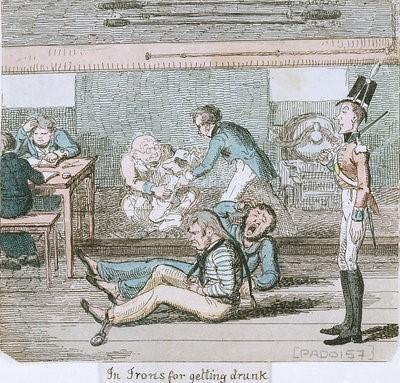
\includegraphics[width=\textwidth]{figures/delgado-img11.jpg}

\caption{\label{fig:key:4.4} “In irons for getting drunk” Colored etching by George Cruikshank}
\end{figure}

Drunkenness was a cultural phenomenon that manifested itself in all ranks aboard ship, not just with the \isi{common sailor}. Because drinking alcohol served a social function, and reinforced \isi{group identity} \citep[13,]{Fury2015} the commanders, captains and officers of maritime communities also regularly consumed alcohol, and also often to excess. Examples of drunken officers in \isi{court testimony} include, “After they had drunke togeather a while Capt Rigby \& George Freebound went on board their vessells againe” [HCA 1/9/3], and “the said captain was so very much in drink that he never was afterwards (according to this Deponent’s best observation) big help” [HCA 1/14/56]; passenger journals describe “the Captain was a very Furious man, and frequently in Drink; so that I could not have opportunity to speak with him” [445f.1/27]; and logbooks corroborate, “Our captn being drunk did quarrel wth me” [HCA 1/99/62] “master drunk at noon” [HCA 1/99/65]. Drunken commanders could pose a serious problem to the social fabric of a shipboard community, for example, in an extended court case against Nicholas Reymer, commander of the ship \textit{Lucy}, in a trial dated June 20th 1682, a witness explains:

\begin{quotation}
Reyner was verry Idle \& most commonly in drink \& he does believe that his seamens disorder were chiefly occasioned by his sole debaucherys \& ill carriage… the dissasters \& damage hapened to the shipp Lucy ...were chiefly occasioned by the carelessness \& disorder of said Reymer \& his company… before \& after the shipp was aground said Raymer was ashoar drinking to excesse  [E134/34Chas2/Mich36]
\end{quotation}

Qualitative data referencing intoxication among the commanding ranks prompts supposition that the harsh treatment sailors experienced at their hands, detailed in \sectref{sec:4.2.2} and tabulated in \tabref{tab:key:4.1} and table 4.2, may have been directly related to their lowered inhibitions as a result of being drunk. However, aside from a few specific cases, we are unlikely to know the true extent of and damage caused by the drinking culture amongst commanders and officers of the period as these privileged few controlled the records and were unlikely to acknowledge blame nor leave evidence that would prompt investigations into their own accountability.

Pirate commanders, and indeed the entire \isi{crew} of \isi{pirate} vessels, are commonly characterized by excessive consumption of alcohol. Although, in extreme circumstances, a \isi{sailor} might lose his allocation of seized goods if he was physically incapable of participating in its capture, e.g., one \isi{sailor} described as “so Drunk they cut him often out of his Share” [HCA 1/99/171], more commonly, alcohol served a vital role in social order and cohesion. Notorious \isi{pirate} captain Edward “Blackbeard” Teach recorded in his personal log the dangers of sobriety among his \isi{crew}:

\begin{quotation}
Such a day, rum all out - our company somewhat sober - a damn’d confusion among us! - rogues aplotting - great talk of separation. So I look’d sharp for a prize - such a day took one, with a great deal of liquor on board, so kept the Company hot, damn’d hot, then all things went well again. (cited in \citealt{Bicheno2012}: 121).
\end{quotation}

Court depositions explicitly associated an inclination for drinking with piracy and accusations were often accompanied by a comment on how much the accused commonly drank, e.g., “for he was a drunken Fellow” [HCA 1/99/103], “he fell to Drinking and became one of the Company” [HCA 1/99/104], “[he] was allways Drunk” [HCA 1/99/116], “he was...very much given to Liquor and was as forward as others at going on Board of Prizes” [HCA 1/99/171], “he knew no more of him than that he loved Drinking” [HCA 1/99/63], and “Deposeth him to be a very Drunken Fellow” [HCA 1/99/158]. Conversely, the case for the defense often pleaded, at best, sobriety, e.g., “Swear him to have been a very Sober, civil Fellow no way mischievous” [HCA 1/99/121], and “never heard him Swear, never given to Drink, and calld Presbyterian for his Sobriety” [HCA 1/99/151], and at worst, coerced inebriation “the pyrates whom he presently Saw were forcing Drink upon him as afterwards they wou’d Some Cloths” [HCA 1/99/147]. The true nature of the situation might be best seen through the eyes of one \isi{sailor} who made his defense against being accused of drinking with a \isi{pirate} \isi{crew}, “As to Drinking he Says t’was aCommon Fault among ‘em, and he knew of no other Company he cou’d keep in that Place” [HCA 1/99/120]. In reality, it may have been that drinking to excess was simply a part of maritime culture and if sailors were to adapt and accommodate to their peers and enjoy the benefits of collective agency and representation, then there was really no alternative than to accept social drinking as part of the lifestyle.  

Maritime communities used alcohol ritualistically to affirm social unity and mark complicity in agreements such as recruitment deals and trade negotiations, few of which were certified by written contacts. \citet{Fury2015} provides evidence of two extreme circumstances in which alcohol was used as a social bonding agent aboard the voyages of the East India Company. The first occurred during the \isi{voyage} of the \textit{Ascension} 1608--9 when Coxswain Nicholas White was convicted of sodomizing the Purser’s Boy, William Acton, and was sentenced to hang; the \isi{crew} passed among them “a cup of wine shared for his farewell” at his execution (\citealt{Fury2015}: 10). The second example occurred on the ship \textit{Good Hope} in 1609 after an uprising led to the murder of Master John Lufkin and, as a result, the men “helped themselves to his provisions, carousing and drinking, toasting each other” (\citealt{Fury2015}: 13). Although superficially there is little connection between these events, the use of alcohol in both serves the role of uniting the \isi{crew} in a gesture of solidarity against what was considered a severe punishment in the first example and as in a gesture of celebration and complicity in the mutinous act in the second. The act of drinking itself served to demonstrate solidarity, as one commander demonstrates in his pledge, “he would not see him wronged in anything and all of the rest said the like Whereupon he called for a bottle of brandy \& Drank wth them and tould them he would make them all men and officers” [HCA 1/101/408-409]. The drinking of the brandy in this example acts to validate the pledge similar to taking an oath or signing a document might if the contract were written. Likewise, the following description of post-trade inebriation seems to be an important part of validating the exchange of goods and strengthens the ties between trading partners for the possibility of future agreements:

\begin{quotation}
One day, a small French sloop came to trade with the English owner of the plantation.  The French smugglers (about fourteen or fifteen men) loaded three barrels of brown (pardo) sugar, eleven sacks of cotton, and one barrel of indigo dye onto their ship, and then left the loaded ship moored while they and the Englishmen they had traded with all got Drunk. \citep[15]{Hatfield2016} 
\end{quotation}

Alcohol served to validate trade agreements and so the taverns and private drinking houses that supplied the alcohol used to validate these deals were not just places to socialize, but offices of maritime business. In the court records relating to one \isi{piracy trial} in Rhode Island and Providence Plantation in 1725, the entire courtroom seems to have moved into a local tavern; the \isi{court clerk} notes “Whereupon the Court adjourned to the \textit{Three Mariners} Tavern… and Opened by proclamation” [HCA 1/99/5]. Yet more commonly, local taverns were not the domain of the administration but rather grassroots maritime communication hubs, e.g. one commander’s proposition to enter into negotiations with another, “the said Brock would be glad to Drinke a Bottell of wine with the said Le Fort that he might have his company” [HCA 1/52/137], and  one letter from a \isi{sailor}’s wife that instructs him “your letter for george herring to be left Mr. Richard merrys here the sine of the \textit{green dragon} nere Shadwell doce [dock] in London” [HCA 1/12/87]. In addition to their role as places of information exchange, taverns were also centers for negotiation on \isi{contraband} trade that was not subject to the monopolies of the Navigation Acts or the restrictions of other European trading regulations. As such, they proliferated in islands that were centers of news networks and trading routes, e.g., “proportionally, at least one in fourteen Bermudian households operated as a part-time tavern” (\citealt{Jarvis2010}: 294). Hatfield’s work on illegal slave trading by English pirates in the \isi{late seventeenth century} as described in Spanish Sanctuary Records suggests the cross-cultural nature of drinking rituals accompanying trade.  She notes that “the French smugglers and English planters caroused together in addition to trading” (\citealt{Hatfield2016}: 17). The international and therefore outlawed nature of such trade may explain why colonial government records abound with regulations against and prosecutions for unlicensed taverns e.g., Barbadian legislation in 1652 “to prevent frequenting of taverns and ale-houses by seamen,” and two years later, the act “prohibiting persons from keeping a common ale-house, or tippling-house, selling any liquors or this country-spirits, to be drank in their houses or plantations without a license\footnote{First legislation dated Jan 10 1652 and the second in the Acts of 1654, both retrieved from the Catalogue of {Acts 1642}-1699, The \isi{Barbados} Department of Archives, St. James.}.” Such legislation may have been an attempt to restrict the flow of information and operations in illegal trade much more than an effort to increase island-wide sobriety, and suggests that local authorities also knew the important role of alcohol in maritime trade negotiations. 

The most extreme and spiritual use of alcohol in maritime ritual relates to preparations among the \isi{crew} before anticipated combat. One witness testimony reports .”..after they had been Drinking all Day togeather towards the evening...to get all together and seize upon the goods” [HCA 1/9/8] and Fury’s research includes a footnote relating to how the \isi{crew} of the \textit{Golden Dragon} drank to each other in a gesture of forgiveness for any wrongdoings and as an act of solidarity before battle (HCA 13/30/108v, cited in \citealt{Fury2015}: 10). The act of drinking before conflict is also referred to in the witness testimony of how one captain and his company prepared for imminent battle “Drinking Rum and Gunpowder” [HCA 1/99 \textit{The American: Weekly Mercury} No.618, Oct 28-Nov 4 1731]. Interestingly, this ritual has historical parallels in Obeah war rituals. Boukman Barima, Professor of Atlantic History and the African Diaspora at Jackson State University, explains:

\begin{quotation}
Obeah’s war rituals survived the erosion of time and were passed like heirlooms between successive generations of freedom fighters as in the practice of consuming rum mixed with gunpowder. Rebels throughout enslavement when they took oaths to pledge their loyalty to each other and their revolt drank this liquid admixture to seal their pact. Binding oaths with liquid concoctions occurs in several West and Central African societies, for instance, in Fanti swearing ceremonies for Omanhene, Asafohene and other leaders this was an essential rite that summoned “the gods to witness” the proceedings and if the person dishonored their pledge “the drink would cause injury or death.” (\citealt{BoukmanBarima2016}: 20 with in-text citations of Shumay’s [2011] \textit{The Fante and the Transatlantic Slave Trade}).
\end{quotation}

The use of alcohol in Obeah war rituals to seal a pledge mirrors the role of alcohol in preparations for combat in maritime, and specifically \isi{pirate} communities, and therefore might also attest to the African cultural influence on such crews. The potential African spiritual influence is even more pronounced when we consider that “common protocol for preparing and hosting rum and gunpowder rituals always demands an adept Obeah man as master of ceremony” (\citealt{BoukmanBarima2016}: 8) suggesting that multicultural crews not only maintained, but also looked towards such spiritual leaders in times of crisis. Hence, regular consumption of alcohol in maritime communities was not just an act of celebration and a necessary replacement for repugnant water supplies, but also served an important role in promoting social order by promoting complicity and unity, regulating trade agreements, and expressing spiritual connectivity in times of distress or anticipated conflict. 

\subsection{{Shared ideologies and leisure activities}}\label{sec:4.2.6}

Sailors were not known for being particularly pious, but the communities they lived in were bound by strong shared ideologies--oftentimes categorized as superstitions, folklore or myths--that manifested themselves in ritual and storytelling. Fantastical beliefs relating to the inherent risks of sailing and the desire for fortuitous sailing conditions date back to antiquity and sailors of the early \isi{colonial period} would have tried to derive meaning from omens and portents in the same way as generations of those that went before them. \citet{Bassett1885} explains in his book on \textit{Legends and Superstitions of the Sea and of Sailors:}

\begin{quotation}
monsters abode in the waters, gods of monstrous shapes ruled them, enchanting sirens, horrid giants, and terrible dragons inhabited the islets and rocks, and on the dry land beyond, there dwelt strange enchantresses, fire-breathing hulls, dwarfish pigmies, and man-eaters….Thus sailors as well as landsmen, in all ages, have been prone to indulge in fancies of all kinds concerning the winds and waves. Such notions are naturally directed to the weather, the object of so much care and solicitude to the \isi{mariner}. \citep[12]{Bassett1885}
\end{quotation}

Eyers asserts that “sailors remain a notoriously superstitious lot” (2011: 5) and his book on nautical myths and superstitions covers material on well-known lore of the sea such as mermaids, the flying Dutchman, evil spirits and ghosts of those departed. Yet, evidence of explicit folklore is rare in archival documentation owing to the nature of the beliefs that were typically transmitted in oral traditions and considered inappropriate to or unworthy of official records; more commonly, official records include references to orthodox religious observations such as the entry “this day being sabath day our Capt was not willing to saile” in the logbook of the \textit{Carlyle} [T/70/1216/9] and the warning by court officials against “being moved \& seduced by the instigation of the Devil” [HCA 1/99 Jamaica {1738}-1739 \& \isi{Bahama} Islands 1722]. However, there are some references to the darker side of sailors’ spirituality in observations such as how one Spanish \isi{crew}: 

\begin{quotation}
began againe to curse and rage against the English which inhabited that Island [Bermuda], saying, that they had inchated that and the rest of those Islands about and did still with the devill raile stormes in those seas when the Spanish Fleet passed that way (\citealt{Gage1648}: 201). 
\end{quotation}

This journal entry demonstrates the sailors’ belief that individuals could enchant the winds and purposefully cause storms, a sentiment famously reflected in Shakespeare’s \textit{The Tempest}, believed to have been written around 1611. Another series of official records which attest to community beliefs in individuals with supernatural powers derive from a series of witness depositions taken in  Virginia 1661, in the case of Robert Clarke [HCA 1/9/51]. Although testimonies do not always align, the majority of witnesses in the case corroborate the beating and ultimate death of Robert Clarke in direct retribution for his necromancy. Testimony describes how Clarke was chained, beaten, had pins thrust into his flesh and was kept from sleeping before being ultimately bound and strangled with a rope around the neck. Deponents explain that his treatment was designed to “beate the Devill out of him...that the devils came often to him and would Speake Softly to him” and “some of the passengers would often call the Said Clarke thiefe \& witch \& the like” and as a result, “Capt Hobbs Did say that they Should never have faire weather till the said Clarke was hanged” [all citations from HCA 1/9/51 batch]. Interestingly, three deponents testify that Clarke was beaten at his own request, had made a confession that he was a witch, could speak Latin, and was often heard reciting the Lord’s Prayer and the Ten Commandments. This suggests that Clarke was an educated man, possibly involved with the church, but who potentially suffered from schizophrenia or some other mental disorder that provoked mass hysteria aboard the ship and tapped into deep-rooted beliefs in supernatural agency on the ships. Certainly, little was known about mental disorder at the time and attacks of epilepsy, aphasia, bipolar disorder, in addition to the effects of degenerative muscle, skin, or mental conditions might very well have been interpreted as something sinister. 

Dramatic rites of passage such as initiation of new sailors when they first crossed the line of the equator commonly bound maritime communities of the early \isi{colonial period}, and the shared ideology of such rituals are manifest even today (\citealt{Bronner2006}). Customs like these expressed solidarities among the \isi{crew} and part of the initiation of new men involved “learning the ropes” when it came to the rites of passage, and so mariners did not customarily make any reference to these events in letters back home or in the official record-keeping. However, owing to the intrigue of one passenger who was privileged to see the custom aboard a \isi{late seventeenth century} Portuguese vessel reports that he witnessed an “ancient custom” which served to initiate any \isi{sailor} crossing the line of the equator for the first time. He describes how the novice \isi{sailor} was required to give food, drink or some physical gift or money equivalent to the mariners, and if any man did not pay: 

\begin{quotation}
the sailors clothed like officers carry him bound to a tribunal, on which a \isi{seaman} is seated in a long robe, who acting the part of a judge, examines him, hears what he has to say, and gives judgement against him to be thrice ducked in the sea after this manner: the person condemned is tied fast with rope, and the other end of it run through a pully at the yard-arm, by which he is hoisted up, and then let run amain three times under water; and there seldom sails to be one or other that gies the rest this diversion. The same is practised in passing the straits of Gibraltar, and the cape of Good Hope. [445f.1/486]. 
\end{quotation}

The dramatic ritual described when crossing the line\footnote{Such rituals are not anticipated to be monolithic but varying among crews and vessels, as such the description serves as an example of one manifestation of the ritual and is not presented as a model.}  includes elements of role play, and specifically the use of costume to reflect the role of the judge, a phenomenon also described and illustrated in Charles \citegen{Johnson1724} description of a mock trial among pirates, see \figref{fig:key:4.5} This practice may have roots in the ancient practices of African and European nations that crowned a king-for-the-day, a role that is still celebrated in carnaval cultures across the Americas and Caribbean islands, and is echoed in the witness testimony of how “the Indian would have command of the vessell and would be called capt: and dailly getting Drunk” [HCA 1/99 Barbados {1733}]. Thus, dramatic role play may have been a salient part of maritime ritual, particularly with regards to using costume to invert social order and play out alternative models of authority. 

Sailors did not always work; they also enjoyed leisure time at sea. The sizeable crews necessitated by navigational, defense, and loading requirements of the large warships and \isi{transatlantic} trading vessels nonetheless became superfluous during favorable sailing conditions and in times of absence of conflict at sea. This was even more notable in \isi{pirate} vessels that maintained a typically larger \isi{crew} and whose \isi{speech community} \citet{Burg2001} compares to the “total institutions” of prisons and mental institutions, characterized by significant leisure time and greater opportunities for extensive social interaction. During such leisure time, sailors told stories, played games, enjoyed music and even staged dramatic performances at sea \citep[155]{Rediker2004} and such speech acts would have provided an ideal situation for the mixing, \isi{leveling} and simplification processes of \isi{new dialect formation}, outlined by \citet{Trudgill1986} and also would have provided opportunities for new recruits to listen to, practice, and acquire features of Ship English.

\begin{figure}
% 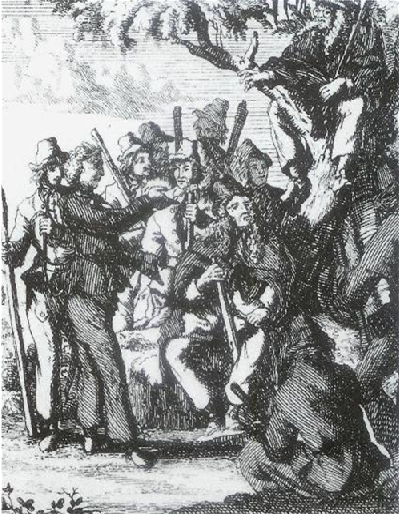
\includegraphics[width=\textwidth]{figures/delgado-img12.png}
\caption{\label{fig:key:4.5} (left) The mock trial performed by the crew of the Thomas Anstis, from Captain Charles Johnson’s \textit{A general history of robberies and murders of the most notorious pyrates} (London 1724) reproduced in \citet[156]{Rediker2004}}
\end{figure}

\begin{figure}
\caption{\label{fig:key:4.6} (right) “Saturday Night at Sea” by George Cruikshank
% , reproduced in \citet[29]{Dibdin1841}
}
\end{figure}

Spontaneous conversation was the most common type of social contact that individual sailors were likely to engage in on a regular basis, and, in the absence of news, gossip and storytelling were favorite group pastimes--as British illustrator George Cruikshank in his “Saturday Night at Sea” (see illustration in \figref{fig:key:4.6}) Participation in storytelling served to strengthen social bonds and maritime traditions, particularly as the repetition of stories also demanded accommodation to the original speaker’s performance style. It is also possible that ships’ cooks, typically older and/or disabled seamen, may have been a focal point of the storytelling tradition, retelling their experiences at sea and teaching new recruits in much the same way as a village elder might. Officer Robert Wilson describes the role of the cook “when their work is finished for the day they’ll take their pipes, seat themselves in Copper Alley, and spin you a long yard [yarn] … about what they have seen and done” (cited in \citealt{AdkinsAdkins2008}: 76). And perhaps it was this very role as the acting village elder that makes the fictional Long John Silver (a disabled cook) so cruel in his attempted corruption of the novice Jim Hawkins in \citegen{Stevenson1883} \textit{Treasure Island}. Sailors knew, as perhaps did Stevenson, that cooks were the focal point of social life aboard ship and their potential role in transmitting language features through narratives in a predominantly oral culture was sacred. 

As mentioned above, music and games were also integral parts of shipboard leisure time, although these often required equipment and some level of experience or ability. Numerous sea shanties of the era survive, not only because regular rhythms facilitated collaborative work efforts, but also because, as Palmer explains, “sailors would assemble there [the mainmast] in good weather during dog-watches and other free times to talk and exchange songs” (1986: xxvii). Repeated references to instruments in witness testimony shows that music featured in the daily lives of sailors beyond vocalizations, e.g., drummers are referred to in various documents [e.g., HCA 1/99/124; HCA 1/14/201; and SP 42/6]. The drum may have served a military purpose, but testimony in cases relating to the forced recruitment of musicians on \isi{pirate} vessels not only  shows that other instruments were on board but also that those who could play them were in high demand, e.g., the accused “took from aubord the Shallop a man belonging to the \isi{deponent} who Could play on the Violin” [HCA 1/99/5], a captured \isi{sailor} “begged hard for his release, insisting on his being a decreped little Fellow unfit for their Purpose, but he was a Trumpeter, and therefore they would not hear him” [HCA 1/99/33], and another \isi{sailor}, “a fidler taken with himself was forced...to sign their articles” [HCA 1/99/49]. 

Similarly, witness testimony shows evidence of equipment used for gaming on board ships, e.g., two sailors arguing over ownership of “Baggamon [backgammon] Tables” [HCA 1/99/81], “Peter Fox abt 25 yeares old... quick and ready of speech, very plausable in Company, a great gamer, and Seldom wthout a ball of dyce in his porkett” [HCA 1/101/411]. Diarists also corroborate the presence of games on board, e.g., Edward Hayes’s \isi{late sixteenth century} journal notes, “we were provided of music in good variety not omitting the least toys, as morris dancers, hobby horse, and May-like conceits” on board the 10-ton frigate \textit{Squirrel} in the \isi{late sixteenth century} (cited in \citealt{Bicheno2012}: 173), and Dr. John Covel’s \isi{late seventeenth century} journal notes:

we seldome fail of some merry fellows in every ship’s \isi{crew} who will entertain us with several diversions, as divers sorts of odde sports and Gambols; sometimes with their homely drolls and Farses, which in thier corrupt language they nickname Interludes; sometimes they dance about the mainmast instead of a maypole, and they have variety of forecastle songs, ridiculous enough (cited in \citealt{Palmer1986}: 104).

Although captains and officers preached the benefits of discipline and self-restraint, they knew that such games were beneficial to occupy idle hands and discouraged more dangerous leisure activities such as talking politics, the conversation about the relative merits of Oliver Cromwell and Charles II that John Barefoot was overheard debating by one witness [HCA 1/9/68]; firing weapons, as happened when pirates got bored and started firing at the \textit{Whydah} for sport [HCA 1/99/99]; and excessive alcohol consumption, discussed in \sectref{sec:4.2.5} corroborated by testimonies such as the deposition that describes the \isi{crew} of the \textit{Elizabeth,} “Carouzing and Drinking with the Rest of the Pyrates” [HCA 1/99/46]. Officers therefore permitted games and music as controlled social acts that helped relieve tedium during uneventful hours at sea. 

Occasionally, ships’ captains would permit (and potentially encourage) more structured leisure activities on board such as theatrical performances. There is evidence that even the lower ranking officers were involved in amateur dramatics, writing, rehearsing and performing plays for visiting officials (\citealt{AdkinsAdkins2008}: 339). Fury refers to “the men included performances of two of Shakespeare’s plays afloat and ashore” on the third \isi{voyage} of the East India Company {1604}-6 (2015: 19). And Gage describes how “for the afternoones sport they had prepared a Copmedy out of famous Lope de Vega, to be acted by some Soldiers, Passengers and some of the younger soft of Fryers” (1648: 16). However, these were likely to have been rare events compared to the more common social activities of telling stories, playing and listening to music, singing songs, dancing, and gambling that fortified the social fabric of the insular ship’s community. 

\section{{Wider maritime communities}}\label{sec:4.3}

In addition to the insular ship communities that each \isi{sailor} belonged to, a wider maritime community encompassed and connected all of the vessels at sea, in port and in river-trade, and also extended to the port and littoral communities in contact with sea-going vessels through local trade, employment opportunities or the service industry. These communities had characteristic features that potentially affected the acquisition and transfer of Ship English and the nature of its internal change, these features included the profusion of maritime contact and the nature of contact in ship-to-ship exchanges, the economic profile of the community that supported a culture of theft and the operation of clandestine networks, and the frequency and nature of contact with port communities. 

\subsection{{Profuse maritime activity}}\label{sec:4.3.1}

Shipping for defense and trade purposes has always been important in Great Britain, surrounded on all sides by the sea. Even as far back as 98AD, a Roman trader described its major port town of London as “a busy emporium for trade and traders” (\citealt{Tacitus1913}), and in the fervor of early colonial manufacture, industry, discovery and international trade, London was defined by its connectivity by sea routes to colonial and foreign locations. \citeauthor{Bicheno2012} explains that the population of London trebled during the \isi{sixteenth century} and in the early \isi{seventeenth century}, the docks of London became “one of the most crowded places on earth... [when] an estimated 75,000 lived in the square mile of the city - which would put it among the top ten most densely populated cities even today” (\citealt{Bicheno2012}: 13). In fact, the Thames was so busy that the lightermen, whose job it was to move cargo and thus make the boats lighter, and watermen, employed to move people and transit goods across the river, made frequent complaints about the congestion around the vast system of docks, wharfs, and warehouses, e.g., in one petition two London watermen complain that “by reason of shipps \& other vesssells continually Lying \& incroaching upon the said staires [landing place] are not onlely greatly hindered in their dayly Imployments but also much ... in their boates which are often splitt \& broken by such vessells” [HCA 1/11/109].  Such complaints led to the 1667 bill under penalty of fine “that no shipp or vessell shall ... obstruct or hinder the passage of any lighter or vessell passing to or from the said dock” [HCA 1/11/140] and speaks to the problems that London’s maritime service providers had to face on a daily basis in the bustling port. 

The importance of the sea in terms of military defense is self-evident for an island-kingdom\footnote{An island-nation after the British loss of Calais in 1558} for whom the seas became, “a moat defensive” in the words of the dying fictional John of Gaunt in Shakespeare’s \textit{Richard II,} (c. 1595, 2.1). \citeauthor{Bicheno2012} explains that “with hundreds of ports and no place more than 70 miles/112 kilometers from the sea, what we might call ‘maritime awareness’ was a constant in English history” (2012: 24). Even at sea, it was a numbers game, Adkins and Adkins explain, “the war at sea was one of attrition, with the navy of each side preying on \isi{merchant} shipping to starve the enemy of supplies, reduce prosperity and thereby limit the capacity to wage war” (2008: 231) and so a profusion of maritime activity was actively encouraged by competing European sea-going nations of the time, and this naturally led to frequent contact between foreign ships in the open waters, evidenced by first-hand testimony, e.g., “[we] Chased a french man of warrr” [ADM 52/2/8], “there was 16 Saile of french” [DDB6/8/4], “a fleet of ships of 14 Saile Supposing them to be a french fleet” [ADM 52/1/8], and “severl Duch Mercht Shipps with a Man of war came in” [ADM 52/2/5]. Frequent contact between ships also happened in busy ports, e.g., a passenger describes the port at Cadiz in 1666:

\begin{quotation}
full of an \isi{infinitive} number of ships, galleys, barks, caravels. tartans, and other vessels, which I was assured at the time amounted to an hundred sail. Just at the entrance of the harbour we saw twenty-five ships of an extraordinary bulk. There is a continual resort of ships from all parts of the world, even from the \textit{Indes}; and it is usual there to see thirty or forty sail come or go out in a day, as if they were but little boats [445f.1/511]. 
\end{quotation}

Such international traffic, in addition to the \isi{transatlantic} \isi{slave trade} that began on a large-scale in the mid-\isi{seventeenth century}, caused crowding in trading zones and the shipping lanes of the open seas because prevailing ocean currents and winds determined ships’ navigation and created international sea-highways that all vessels were obliged to use (\citealt{AdkinsAdkins2008}: xxxiv and refer back to \figref{fig:key:4.1}] As such, and according to the British National Maritime Museum’s information on shipping lanes, “they also determined the nature of maritime trade and social interaction” (Atlantic Worlds exhibition, Nov 22 2015).  

Shipping, critical to the home-based defensive and trading hubs of England, was perhaps more crucial to interconnected colonial settlements. Since the fifteenth century rise in the cod market, the annual fishing migration to Newfoundland saw the English and French fight over control of the port settlements. And with the sixteenth-century demand for oil to use in lamps and bone for manufactured goods such as corsets, umbrellas, shoe-horns, and fishing rods, whaling activities increased in international waters and prompted conflict over the ports that lay on whaling migration routes. The seventeenth-century land grab in the Americas and the Caribbean and the plunder of labor from Africa saw associated movements of officials, merchants, missionaries, military, workers, settlers and captives across the waters and around the colonies. The military presence needed to secure these new colonial holdings meant that the mid-\isi{seventeenth century} was a time of exponential maritime growth for Britain. Linebaugh and Rediker explain, “the Navy had 50 ships and 9,500 sailors in 1633, and 173 ships and 42,000 sailors in 1688” (2000: 146).  The number of ships continued to grow, reaching more than five times the size of the mid-\isi{seventeenth century} fleet with 939 ships registered in 1815 (The National Maritime Museum, “Nelson Navy Nation.”) 

This period also saw a growth in the range and connectivity among colonial ports, perhaps best illustrated by a summary of the shipping news in \textit{The American: Weekly Mercury} [no. 617--618] covering the period of two weeks from October 21 to November 4 1731, in which 79 percent of the vessels in port were arriving from, or bound to colonial territories compared to twelve percent from/to foreign ports and only five percent heading from/to Great Britain (see \tabref{tab:key:4.3}) Ships such as the \textit{Antelope} were kept in constant transit around the colonies, e.g., logbook entries from 10 June {1690} to August 3 1691 detail consecutive voyages around Montserrat, Nevis, St. Christopher, Santo Domingo, Antigua, \isi{Barbados}, Martinique, Rhode Island, Guadalupe, and Carlisle Bay covering a period just over one year [ADM 52/1/7]. Such voyages were reflective of a phenomenon in which colonies became more autonomous and leveraged the trading commodities, workforce, and defensive capacities that local trading partners could offer before seeking to engage with the customs regulation and high duties that trade and transit with Britain incurred. However, the statistics recovered here are only a partial account of all the traffic that was operating among the colonies. The smaller craft that were critical for day-to-day operations and essential in the inter-colonial networks of trade and communication often bypassed British record-keeping efforts. \citeauthor{Jarvis2010} explains that large ships were much less common compared to the ubiquitous smaller vessels of intercolonial traffic and presents a table of vessels clearing North American ports in 1772 showing only 2,149 large topsail vessels (just under 30\% of the total traffic) compared to 5,047 smaller sloops and schooners (over 70\% of the total traffic) (2010: 122--123, Table 4). 

\begin{figure}
\caption{\label{tab:key:4.3} Summary of shipping information for New York and Philadelphia covering the period of two weeks (Oct 21-Nov 4) in 1731, based on data in HCA 1/99, \textit{The American: Weekly Mercury} (no. 617--618)}
% \includegraphics[width=\textwidth]{figures/delgado-img14.wmf}
\end{figure}
 

He also comments that, even when vessels registered with British authorities, “harried customs officers had neither the time nor the resources to verify information in the registers that mariners presented” (\citealt{Jarvis2010}: 159). Hence, and accepting the difficulties of data collection in a context of covert trade and falsification of customs records, records suggest that colonial ports saw intense maritime activity, much of which was inter-colonial in nature rather than \isi{transatlantic}. 

Profuse activity around colonial ports attracted \isi{contraband} trade and piracy which created additional traffic in the shipping lanes. \citeauthor{Gage1648}’s description of a colonial port in the Spanish Americas in the mid-\isi{sixteenth century} shows how a typical “sea towne” was populated, “some very rich Merchants dwell in it, who trade with Mexico, Peru, and Philippines, sending their small vessles out from Port to Port, which come home richly laden with the Commodities of all the Southerne or Easterne parts” (1648: 88). And in such a context, it is clear why British sailors seeking the easy pickings of the Spanish Empire in South America were attracted to the commodity-rich and defense-poor port towns of the colonial Atlantic. British colonies were also targets for foreign raids and the attempts of pirates who rejected any national alliance. In the \isi{late seventeenth century}, Virginia Governor Francis Nicholson was so keen to secure safe shipping that he offered bounty money for the capture of specific pirates, and “if it was not allowed in the publick Accounts, his excellency was pleased to say, he would pay it him self” [CO 5/1411/644]. Similarly indicating preoccupation with the proliferation of piracy, although eight bills were discussed relating to the administration of the colony of Virginia on 22 May {1699}, e.g. export duties on food, treatment of colonists, regulation of the judicial system, treatment of wildlife, and the regulation of the economy, the first bill to be discussed and approved was the “bill for restraining \& Punishing pirats and Privateers,” suggesting that it was a more pressing topic of concern than the local food supply chain, wellbeing of settlers, or the economy. The issue of piracy was also discussed in full assembly only four days later on 26 May before the less-urgent matter of a bill against “unreasonable killing of poor” [CO 5/1411]; and it was not until the following month that the assembly met to discuss “a bill for building the capitol \& the city of williamsburg” [CO 5/1411/77]. Without first safeguarding the shipping lanes, the administrators of Virginia knew, as did their contemporaries, that there was no point in developing a settlement. 

\subsection{{Convoys and communication}}\label{sec:4.3.2}

Transatlantic vessels frequently travelled in \isi{convoy} for protection against foreign and \isi{pirate} attack, and communication among these convoys was a regular feature of \isi{language contact} in \isi{maritime speech} communities. Of the 27 recoverable references to a specific number of vessels sailing in \isi{convoy} with a majority of British sailors, the average number is 22 ships per \isi{convoy}. The highest number is 92 [DDB6 8/4] but this seems to be an exception to the trend of convoys numbering between 15 and 30 ships that were most common in international waters (see \figref{fig:key:4.7}) 

\begin{figure}
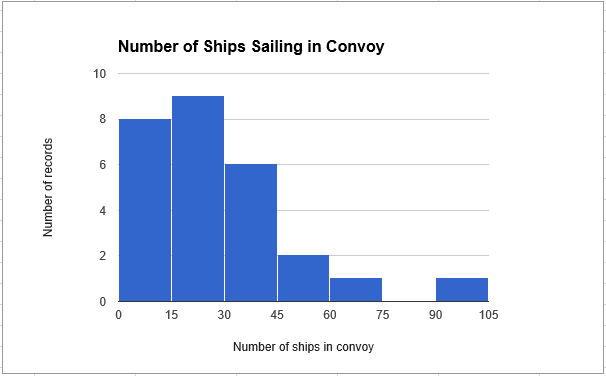
\includegraphics[width=\textwidth]{figures/delgado-img15.png}
\caption{\label{fig:key:4.7} Number of ships sailing in convoy based on witness depositions, logbooks and journals\textsuperscript{a}}

\textsuperscript{a} Sources: SP 42/6, DDB6 8/4, CO 5/1411/664, ADM 52/2/5-8, HCA 51/3983/1, ADM 52/3/7, 13, ADM 51/4322/4, ADM 51/3954, HCA 1/99/26, HCA 1/99/3/6, HCA 1/98/45,47, DDB6 8/4, MMM BL/Egerton 2395/0003, \citealt{Bicheno2012}: 183, \citealt{Gage1648}: 11, 15
\end{figure}

Much larger groupings of ships were possible in port, e.g., “an hundred sail” and “five hundred...fishing boats” [445f.1/511] yet as such references do not necessarily imply that any of the vessels sailed in \isi{convoy}, they are not included in the data composing the graph in \figref{fig:key:4.7} The vessels that evidence indicates did sail in \isi{convoy} with others were potentially made up of mixed groups at sea, both in terms of vessel size and a range of \isi{merchant} and naval vessels e.g., “above 22 sail with 3 \isi{merchant} Ships \& Sloopes” [ADM 52/1/7], “seven ships \& one sloop going after \& 10 long ships" [HCA 1/99/26], and “seven large and 22 small ships” (\citealt{Bicheno2012}: 183). The common maritime practice of sailing in convoys for safety and increased force in the event of attack was also evident among foreign nations, e.g., “16 Saile of french” [DDB6 8/4], and “the Dutch were being about 60 Sayle of men of war” [ADM 52/2/5]; and also in groups composed of international allies, e.g., “the \textit{Assurance} with 12 English Marchant men 2 dutch men of warr \& 30 saile of marchant men” [HCA 51/3983/1]. Just like the naval and \isi{merchant} traditions they grew out of, \isi{pirate} communities also collaborated in \isi{convoy} (\citealt{Esquemelin1678}; \citealt{Rediker1987}: 268) making the feature of this type of collaboration something that characterized all types of \isi{transatlantic} maritime communities during the early \isi{colonial period}. 

Some fleets may have sailed in perpetual and planned \isi{convoy}, but many convoys formed at sea without prior organization. \citeauthor{Bicheno2012} explains how throughout the \isi{sixteenth century}, maritime activity evolved “from shoal to school” (2012: 51), and as part of this development, ships started sailing in convoys more. He gives examples of some of the planned convoys of the \isi{late sixteenth century} in which “articles of consortship” established spacing between ships at about six miles / ten kilometers from each other on a south-north axis (\citealt{Bicheno2012}: 305). However, into the \isi{seventeenth century} and the profuse maritime activity that came with multitudes of private traders now able to navigate the \isi{transatlantic} passage, convoys were not always planned from the outset but formed as opportunities arose; or, as one contemporary succinctly puts it, “they met at sea” [HCA 1/14/203]. For this reason, willingness to sail in \isi{convoy} was sometimes mandated in captain’s instructions, e.g., one letter from the Admiralty dated 5 December {1699} to Captain Aldred, Commander of the \textit{\isi{Essex} Enterprize}, instructs “give Convoy to any other ships or vessels of his Majestys subjects bound your way, which shall be ready to sail with you, or you shall meet with, as far as your way shall lie together” [CO 5/1411/657]. And instructions like these confirm that convoys formed impromptu at sea and likely lasted as the participants found mutual benefit in shared passage, as described in one witness testimony regarding a vessel from Newfoundland that “willing to Consirt wth us in our Design and soe Proceeded wth us” [HCA 1/12/1]. Journals and logbooks show evidence of how vessels left convoys after they ceased to be beneficial e.g., “the eight Galeons took their leave of us, and left our Merchant ships now to Shift for themselves” \citep[15,]{Gage1648} “this morning mett three East India Shipp which we toke In our Convoye” [ADM 52/1/1], and “we lost Company of 10 ships \& Supposed they Staied moord” [ADM 52/2/8]; note that in the last quotation the word “supposed” indicates that there was no prior agreement and that the ships composing the \isi{convoy} sailed independently. It was therefore possible that multiple convoys were operating in the busy sea-lanes and that vessels could effectively tack from one to the other, as illustrated by one \isi{sailor}’s observation, “wee have sayled \& Loggd \textit{upon severall Covoyes} 44 miles” [HCA 51/3983/1, emphasis added].  Such networks of convoys potentially gave rise to a kind of maritime underground railroad for rebels, escaped slaves and indentured workers, a suggestion that might explain the deposition of Alexander Wyat who testifies that two sailors promised to get him away from Havana to France [HCA 1/99 \isi{Bahama} Islands 1722], another runaway who “got on Board a Dutch Ship” [HCA 1/99/171], and a letter regarding “a mollatto” that ran away and whose likely movements are described:

\begin{quotation}
he gott to Road Island and perhaps is gon from thence with som of the pryvateers that fitted out there for the Gulph of Porlya... If hee bee, it’s not unlikely but he is or has been att the marys or Maddagascar [HCA 1/98/75]. 
\end{quotation}

The proven existence of such maritime railroads undoubtedly requires further research, but the common maritime practice of sailing in \isi{convoy} that was observed throughout the period under study certainly indicates that encounters at sea and consequent impromptu convoys between vessels formed a wider community of sailors on the open waters. 

The practice of forming unplanned convoys necessitated communication between vessels, if nothing more, to establish an unknown vessel’s purpose and destination in addition to the captain’s disposition to sail in consort. As a result, records of the era are replete with notes relating to chance encounters with ships and efforts to communicate with them, e.g., “one day we discovered a ship, and it being our captain’s duty to know what she was, he made all the sail he could” [445f.1/511], “we espied a ship...being within 3 leagues of it we tackt \& speak with the ship” [ADM 52/1/7], “[a ship] bounde for Newfounde Lande: one of our fleet speak with them” [ADM 52/2/8], and “we had sight of a ship and about three she Bore to us... to speak with us” [T/70/1216/13]. In order to initiate communication, crews often used signals that would be transmitted over larger distances, such as flags, guns, and fanfare, e.g., “putting out English colours invited the \textit{Maliver} to come and pate [talk]” [HCA 1/53/13], “to give notice to our fleet...wee fired 3 gunes Distance and ...a muskett” [HCA 51/3983/1], “hee Came upon us at a distance \& spread his Dutch collors then wee fired a gun [of salutation] at him soe hee Came unboard us” [HCA 51/3983/1], and “the other vessels bore up to us, and gave us a consort of drums and trumpets, saluting us with three huzza’s all the sailors gave, taking the signal from the boatswain’s whistle”  [445f.1/510]. If the vessels were broadside or near enough, then sailors might call to each other from deck to deck or across the gunports, e.g., “[a \isi{sailor}] did what hee could to speak with mee, being within halfe a mile of mee” [ADM 51/3954], “they hailed him and they spoke with one another” [CO 5/1411/99], and “the whole morning was spent in friendly acclamations and salutations from ship to ship...Sea greetings” (\citealt{Gage1648}: 201). Yet sailors also frequently used small craft to visit each other’s vessels, described as “visiting each other with their Cock-boates” (\citealt{Gage1648}: 15).  Officers, in particular, were required to visit other ships as part of proper custom and in order to collaborate with other officers in the fleet, as illustrated by the references: Captains Snapes and Hawkes daily came on board and returned to their own ships [SP 42/6], “this morn a Councill of war on board the \textit{Dutches}” [ADM 52/2/5], and “a Consultation of Flagg officers held on board the \textit{Britania}” [ADM 52/2/5]. Yet the common sailors also had opportunities to pay their peers ship-visits, albeit without the ritual pomp, e.g., “one Mariner of the ship called \textit{St. Francisco} being more [ad]venturous than the rest, and offering to swimme from his ship, to see some friends in another not farre off\footnote{This attempt was not very successful however as the swimmer became “a most unfortunate prey to one of them [sharks] ...who had devoured a leg, and arme, and part of his shoulder” \citep[21]{Gage1648} perhaps explaining sailors’ characteristic reluctance to swim.}” \citep[21,]{Gage1648} and Abel Taylor’s testimony that “2 or 3 times every day that weather would permitt [them to get] on board [another ship]… and this he declared was practized as well at sea as at Malago \& in other parts \& that he hath known” [SP 42/6/29]. \citeauthor{AdkinsAdkins2008} suggest that \isi{crew} visits were a common form of leisure, “although the seamen were only occasionally given shore leave, they were generally permitted to visit other nearby ships on Sundays” (2008: 349). Ship to ship contact provided the networks by which many sailors kept in touch with their families, e.g., one wife’s expectation that “this [letter] will God Willing Come to your hands by the ship \textit{Katheryn}” [HCA 1/98/58], and was also a means to seek and disseminate news of maritime movements, e.g., “in the evening speak with the \textit{Katherine} Yatch who told us the Flemmings were gone to the Westward” [ADM 52/2/6], “a small pinke came up with us \& said shee saw the \textit{Assurance} tack in the night” [HCA 51/3983/1], and “Last night Arrived a Small bark \& a sloop for the Antego that brings news of the \textit{Garsey} being taken” [ADM 52/1/8]. In fact, getting news from other ships was so common that when it did not happen, it was more likely to be noteworthy, e.g., in the logbook of the \textit{Antelope} 6 March {1691} “this morning arrived here a hag boat from London [that] brought little or noe news at all” [ADM 52/1/8]. And although we only have witness accounts of such contact between vessels for the majority period under study, later the \textit{Lloyd's List} would report on such “speakings” that were records of communication between ships that met at sea. In short, interpersonal and symbolic communication among the vessels in convoys served a vital function in maritime collaboration; it provided opportunities for sailors to socialize, organize, and collaborate in a way that strengthened the networks of maritime connectivity across open waters and potentially also aided \isi{language transfer} around these extended communities in stark contrast to the literary trope of the lone boat at sea sailing for months without contact that Samuel Taylor Coleridge popularized in his (1798) \textit{Rime of the Ancient Mariner.} 

\subsection{{The colonial maritime economy}}\label{sec:4.3.3}
\largerpage
  Fishing and cargo-shipping formed the basis of Britain’s trading economy with foreign neighbors since the first sailors crossed the channels to modern day Ireland and France, and with the advent of more reliable \isi{transatlantic} passages in the \isi{sixteenth century}, sailors forged the intricate mercantile networks of international commerce on a much greater scale. In {1562}, and with the backing of Elizabeth I, Hawkins challenged the Iberian monopoly on the \isi{slave trade} when he shipped African captives to Hispaniola, and Charles II furthered Britain’s involvement in this form of human trafficking with a charter to the Royal Adventurers of England Trading into Africa in 1662 (\citealt{Brown2011}: 105). Around the same time, Britain was fighting the Dutch for commercial supremacy off the south coast of England, culminating in the Navigation Acts of 1651 that were explicitly designed to maintain trade monopolies in the face of international free markets (\citealt{Brown2011}: 41). As the British stronghold on colonial commerce increased, so did its role in the transit and sale of human cargo around the Caribbean and Americas. For example, \isi{Liverpool}’s first known slave ship set sail in 1699 and carried 220 captives from West Africa to \isi{Barbados}, and by 1750 slaving voyages from \isi{Liverpool} dominated the trade, significantly outnumbering those from London and Bristol, controlling over 80\% of the British trade and more than 40\% of the European market by the turn of the century\footnote{Merseyside Maritime Museum Archives \& Library. (2014) \textit{\isi{Liverpool} and the Atlantic Slave Trade} (Information Sheet: 3). Retrieved from \url{http://www.liverpoolmuseums.org.uk/maritime/archive/sheet/3}}. 
  Various depositions of the \isi{seventeenth century} refer to the infrastructure of this trade around the Atlantic, specifically “factories” and “agents” in West Africa that functioned not only in horrific sites of brutality and abuse, but also created points of commerce [HCA 1/12/2-4]. These points of commercial contact involved \isi{language contact}, potentially giving rise to the development of what Hancock describes as a “Coastal English” (\citealt{Hancock1986}; \citealt{DelgadoHancock2017}).

In addition to trade in foodstuffs, manufactured goods, and human trafficking, sailors were also essential in maintaining the economies of war by moving large numbers of troops, equipment, and captives during regional wars. For example, Taylor’s diary gives details of maritime involvement in the 1691 surrender of Limerick:

\begin{quotation}
to facilitate the Transporting of the Troops, there General will furnish 50 Ships, and each Ship Burthen 200 Tuns… and also give Two men of War to imbark the Principal Officers , and serve for a Convoy to the Vessels of Burthen.…And if there be any more Men to be Transported, than can be carried off in the said 50 Ships...where they shall remain until the other 20 Ships are ready, which are to be in a Months time; and may imbark in any French Ship, that may come in the mean time. [HCA 1/13/122.]
\end{quotation}

In addition to legitimate maritime transit and commerce, sailors also supplied colonies and regions around Great Britain by keeping open channels of smuggling for \isi{contraband} that was often hidden in vessels with false bulkheads, hollow spars, and adapted cavities between decks\footnote{Merseyside Maritime Museum Archives \& Library. (2010)  \textit{History of Rummage} (Information Sheet: 73). Retrieved from \url{http://www.liverpoolmuseums.org.uk/maritime/archive/sheet/73}}. In this context, sailors made the most of opportunistic trading, as described by one witness, “wee sailed along the coast and fell in with the river Sesters and theire wooded and wattered and Traded wth the negroes for fresh provisions” [HCA 1/12/2]. It was precisely this type of ad hoc trading that potentially led to the development of English pidgins around the multilingual coastal regions of the Americas, the Caribbean and Africa. Illegal trading became so intense around \isi{pirate} havens like Port Royal, Tortuga, Providence and Madagascar that the collusion of any unknown vessel was assumed, prompting one captain leading a trading \isi{voyage} around \isi{Jamaica} in 1698 to go to the trouble of getting a letter bearing a seal from the governor that assured all readers of “his just and lawfull affairs” and urging port officials to give his ship free access [HCA 1/98/53]. However, lawful affairs were not everybody’s intention and heavy-handed measures against piracy were taken in the early \isi{colonial period} to limit damage to the local economy caused by proliferating networks of \isi{contraband}. In fact, upon close attention to the wording of trials against pirates, it seems that the authorities were far more concerned about the hazard to the economy that these people presented rather than the protection of basic human rights, as illustrated in the wording of one statement used to open proceedings in a \isi{piracy trial} in \isi{Barbados} in 1733: “the crimes of piracy, felony, robbery, \& murder committed on the sea are most odious and detestable, \textit{being destructive of all trade and commerce}" [HCA 1/99 Barbados {1733}, emphasis added]. Yet, all sailors of the early \isi{colonial period} performed critical service roles in the British and regional economies not only when they operated under legal jurisdiction but also when they developed prohibited networks of debt, credit and communication that shaped both economic and linguistic developments in the decades and centuries to come. 

Mariners operated largely on \isi{barter} economies because coined money was limited and often useless in the context of unregulated international trade. British legal tender was so scarce that sometimes the payment of debts in cash appears to be a notable event, e.g., court cases that refer to “two hundred pounds lawfull money” [HCA 1/9/7], “five pounds payd him in money” [HCA 1/9/64], and “paid him in money” [HCA 1/9/67]. Some trials show evidence that Spanish currency was used, e.g., court proceedings, relating to the theft of “a certain kind, Or pieces or species of money comonly Called pieces of eight to the value of One hundred pounds of lawful money of great Britain” [HCA 1/99/7] and description of trade in Tunis using “some Spanish doubleloons...knowing how scarse money was" [SP 42/6]. Yet, more commonly witness statements attest to \isi{barter} economies in lieu of monetary exchange, e.g., the \isi{voyage} that took on slaves, flour, beef, and sugar in Antigua to trade for stickfish and wood in Curaçao [SP 42/6], the exchange of “one negroe man slave and five shift for anchorage and seventy pieces of eight in lieu of a barrell of serviceable powder” [HCA 1/98/77], and the invoice of dry goods consigned to Capt Samuel Burgess with the instruction “to sell for my more advantage [or.].. to lay it out in Such goods or merchandise as you shall think will turn to the best advantage here” [HCA 1/98/143]. There is evidence that salt may have been the preferred currency in Atlantic \isi{barter} economies when the access to and value of European currencies collapsed at various points in the early \isi{colonial period} (\citealt{Jarvis2010}: 400). Dampier gives a first-hand testimony of how this might have worked in maritime trading, “I told him I had not Mony, but would exchange some of the Salt which I brought from Mayo for their Commodities. He reply’d, that Salt was indeed an acceptable Commodity” [1045.f.3/1/31: 30]. Furthermore, \citeauthor{AdkinsAdkins2008} suggest that the use of food items and clothing as currency was also a common feature of trade both in port and among \isi{crew} (2008: 97, 122), e.g., four sailors testify how their captain paid them in shoes and stockings with the explanation that they could trade with these items as if they were money [SP 42/6] and another testimony explains “if the said master would not give them five crownes he would take 1000 hundred fish for the said shott” [HCA 1/101/431]. Interestingly, the use of salt, clothes or foodstuffs as currency may have some connections with trading economies in Africa that bartered with cloth and shells [445f.1/491-2; \citealt{HogendornJohnson2003}]. It may very well be that sailors’ participation in \isi{barter} economies and their use of dry goods and provisions as currency in trade was something reinforced by contact with West African societies, much like their use of language may have accommodated African forms of speech. 

Systems of credit, debt and loan also served to enable trade and strengthen Atlantic networks of reciprocity. Often, credit was extended in partial payment alongside \isi{barter} deals, e.g., one letter to the British ambassador to Spain explains how “money is not to be got at Havana for the Negroes” instead, they sold on credit and took crops as a percent of the debt (\citealt{O’Malley2016}: 20). At other times, one party would loan money to enable trade under conditions of return, e.g., \isi{merchant} Robert Balle testified in 1682 that he lent commander Nicholas Reymer various sums of money for ship repairs, under the understanding that when the ship put into port in London, the money would be repaid [E134/34Chas2/Mich36], and rope maker Samuel Sherman testified in 1636 that he lent the Boatswain of the \textit{Andrew} some money that he repaid in rope and barrels of tar “as pawne for his debte untill the examinnat has recovered his wage to paie him” [HCA 1/101/221, 224]. Yet, in spite of sailors’ promises to be “punctuall \& just in the payments” [HCA 1/101/546], many parties ended up in court when they failed to pay debts or when they attempted payment in unacceptable terms such as Captain Williams’ hand-written twenty pound note that was rejected because “Notes of Hand signed at Sea were not valid” [HCA 1/99* \textit{The American: Weekly Mercury} No.618, Oct 28-Nov 4 1731]. Yet when merchants, captains, vessel owners and service providers complied with their debt obligations they constructed international webs of commerce based on trust and mutual benefit that perpetuated local economies and laid the foundations of emerging international economies. 

\subsection{{Corruption and theft}}\label{sec:4.3.4}

Despite their massive contributions to European and colonial economies, sailors of the colonial Americas, Caribbean and Africa operated cultures of theft in which ideologies of personal gain were more commonplace than conscientious acts of nation-building. Indeed, such ideologies proliferated in the British colonies themselves among corrupt governors and officials operating public and clandestine networks dedicated to personal gain and often at the expense of others. Even though the mother country provided an abundance of models and examples in this nefarious domain, \citet{Fusaro2015} explains how these colonial spaces were ideal regions which favored autonomy and enabled self-interested parties to operate nefarious schemes at a distance from imperial oversight. Examples recovered from the archives include: Bermudian councilors debated British mandates and voted on whether or not to enforce clauses they disliked \citep[55]{Jarvis2010}; governors of Martinique and Guadeloupe encouraged captains to ignore strict rules against trade with France and bring slaves into their labor force (\citealt{O’Malley2016}: 9--18); corrupt officials in Anguilla, Nevis, and other British islands gave vessels permission and protections to unload \isi{contraband} cargoes openly \citep[173]{Jarvis2010}; and officials in Newfoundland took bribes to reserve port spaces, operated complex scams to dupe sailors from their pay, took settlers and natives hostage for ransom, and forged “certificates of clandestinity”\footnote{Although no surviving examples of “certificates of Clandestinity” survive in the archive, various references to them in the series SP 42/6 suggest that they were letters of agreement to unlawful practices that were passed around specific ships’ officers to mark their agreement and complicity in nefarious activities. In this same document series, certain illiterate officers testify to signing the certificate without knowing what it was and others testify to not having seen or signed any such certificate.}  among illiterate ship masters to cover for their own abuses of authority [SP 42/6]. The reference to a distinct “coast price” in one witness testimony describing “the goods…[that] amounted to the Value of Twenty Pounds at the Coast Price” [HCA 1/99 Cape Coast of Africa, Feb 4 1734, 4] also implies that coastal regions were subject to potentially inflated prices that included bribes and semi-official “taxes” on imported goods that no doubt went directly to government officials. Sir Robert Robinson, Bermuda’s governor from 1687--1691, was one local official who personally benefitted from such suspect practices. Robinson made “a small illicit fortune from bribes, fees, and embezzled duties and public funds” \citep[70]{Jarvis2010} and was one of the many unqualified and incompetent colonial administrators characterized by upholding unscrupulous, discriminatory, and self-interested practices. His background as an ex-navy captain, like many colonial governors, also illustrates the profound links to corruption among maritime communities and colonial administration.

The maritime culture of theft and self-interest negatively impacted the British government’s hold on colonial commerce, but ironically, it was fifteenth and \isi{sixteenth century} British corruption that prompted many of these ideologies among maritime communities in the first place. \citeauthor{Bicheno2012} explains how the House of Tudor, and specifically Elizabeth I’s state, was dependent on traditions of piracy that enabled the monarch to collect unofficial taxes on traffic in illicit goods to fill the national coffers. As a result, \isi{sixteenth century} state-sponsored piracy in the form of corsair activity and privateering proliferated and private pirate-entrepreneurs such as Sir Walter Raleigh and George Clifford, Earl of Cumberland, operated with the queen’s knowledge and approval (2012: 134--328). The very fact that Francis \isi{Drake} was knighted in 1581 in England but remains known as a \isi{pirate} in the Spanish-speaking Caribbean\footnote{Born in England, I learned about “Sir Francis \isi{Drake}” in school and through cultural transmission. I was shocked to hear him referred to as “The Pirate \isi{Drake}” in an English-language commentary accompanying a video in San Juan’s \textit{El Morro} when I first arrived in Puerto Rico in 2006.}  indicates the range of conflicting ideologies related to the service of sailors.  Moreover, that the exploits of such men no longer feature on British schools’ curricula speaks to the fact that they were “the sharp-edged products of a far more abrasive age” (\citealt{Bicheno2012}: 327). As a result, in 1603 James I inherited a \isi{pirate} nation whose allegiance to Britain was far weaker than its allegiance to profit, and consequently more cargoes and ships were lost to British pirates preying on their home state than to foreign attack during the Spanish wars (\citealt{Bicheno2012}: 328). The monarch’s efforts to regulate and reign in the renegade maritime communities consequently led to all-out war at sea in the \isi{seventeenth century} which only began to settle after the state’s complete rejection and suppression of piracy in the early \isi{eighteenth century}. 

Cultures of theft and abuses of power not only prevailed in the British and colonial governments but also much more specifically among the naval administration and regulating bodies of the \isi{merchant} services. \citeauthor{Bicheno2012} explains that “the self-financing power vested in the Admiralty Commission invited the extortion and other abuses that came to characterize the office” (2012: 158) and \citeauthor{Lincoln2015} further explains that by the time of Pepys’ administration, reforms to stop fraudulence in the Admiralty, and specifically in shipboard accounting, were long overdue because of a culture in which “national duty and private gain were not mutually exclusive” (2015: 145). Naval spending was directed to preferred contractors and commonly involved deals susceptible to nepotism, bribery and fraud. In such a context, it is understandable that naval commanders, captains and senior officers often bypassed legal or moral protocols to make a profit, e.g., senior officers taking cargo such as cloth, raw hides, and sugar for private sale and stealing bags of money [SP 42/6], a superior officer instructing a subordinate to make holes in the bottom of a heavily good-laden ship to feign the sinking of the ship, scare away the \isi{crew}, and allow him free-access to the cargo [HCA 1/12/84], a quartermaster helping himself to \isi{crew} supplies [HCA 1/99/90], a lieutenant forging official documents [ADM 106/300/54], a captain bribing officers to keep quiet about what they had seen [HCA 1/99/130], a captain submitting unsigned and incomplete customs documents [CO 5/1411/653], and the common practice of pursers skimming off provisions (\citealt{AdkinsAdkins2008}: 32).  For such reasons, attempts to combat corruption were necessary, e.g., instructions to one captain that explicitly forbade him from taking his pick of the cargo before any captured prize was officially processed [HCA 1/9/19], a letter thanking the naval board for money and assuring them that the officer in charge would “see to prevent any abuse” [ADM 106/300/91], an opening statement in court explaining “the duty of Masters of ships, and the great trust that is put into their hands, upon the account of their Merchants and Owners; and what damage and Frauds and Felonies at Sea do bring upon all Foreign Trade and Commerce” [HCA 1/12/111], and a letter sent to captains from one governor‘s office promoting “a due observance of the several acts of Trade made for preventing frauds \& regulating abuses” [CO 5/1411/618]. Corrupt officers, the self-described “Gentlemen of fortune” [HCA 1/99/6], abounded in a maritime culture of corruption, and as such, it is not difficult to see how armed piracy evolved in the late seventeenth and early eighteenth centuries in reaction to officious legislation that attempted to regulate and reap national profits from the accepted and individually gainful practices of earlier times. 

Sailors stole for personal gain but also for survival. Given the maritime culture of theft that permeated the administration and commanding ranks of the vessels, it is not surprising to see evidence of individual counts of theft among the common men, e.g., one letter describing a crewman who “was robbed on Saturday last at night of about six pounds seventeen shillings” by some of his peers [ADM 106/288/46, 48] a deposition about another \isi{sailor} who is convicted of “the Embezzlement of sundry Goods out of the Longboat belonging to the Servant of Bristol” [HCA 1/99/6], and a logbook entry “this morning...Jacob Annis was whipped at the Maine Yeard for Breaking open a Chest and Takeing out moneys” [ADM 52/3/7]. The “chest” referred to in the previous citation was the only individual space permitted to the \isi{common sailor} and the theft of personal items, referred to as the “hauling and Plundering of Chests” [HCA 1/99/105], occurred with enough frequency when ships were captured at sea that one captain comments “there was not an honest man in yarmouth,” a common recruitment site for seamen [HCA 1/101/431]. Yet sailors were not necessarily interested in money or items to sell, they also plundered chests for essential items such as clothes that were difficult to acquire and impossible to manufacture at sea, e.g., “the \isi{prisoner} in Particular has Some of his cloths... of which he returnd only a shirt” [HCA 1/99/93], “he was shifted with a shirt he knew was not his own” [HCA 1/99/99], “Did make away as likewise your petitoners Sons clothes” [HCA 1/11/110], and “taking from the said John Wingfield his wearing apparel” [HCA 1/99/170]. 

Theft at sea happened on an individual and collective scale. Individuals stole what they could for personal reasons, e.g., “they saw him rummaging their Surgeon’s chest [HCA 1/99/81], and “they went into a cabbin and tooke a piece of cold beef and Cabbidge and some Bisketts” [HCA 1/53/68]. Crews also plundered captured vessels for the necessary materials to keep their vessels and their workers functional, e.g., records attest to crews targeting ships and plundering captured vessels for such things as: food and provisions [HCA 1/99 \isi{Bahama} Islands 1722]; sails and canvas [HCA 1/99/50; HCA 1/99/125]; rigging, anchors and cables [CO 5/1411/631]; and masts, yards, ropes, cords and tackle [HCA 1/101/351]. Captains were also keen to recover any materials found afloat or washed ashore that might be gainfully used, as illustrated in the need for a man “eimployed to looke after stolen or drift goods" [ADM 106/288/33]. Thus, although many crews and individuals may have been motivated to plunder for personal gain, there is significant evidence that theft at sea was also motivated on a larger scale by necessity in harsh conditions. 

Rather than envisioning a simplistic division between piracy and legitimate trade, there seemed to have existed a continuum that ranged from violent theft, through forced trade and coercion, to free but non-legitimate commerce that formed an important part of local colonial economies. Indeed, the following letter dated 1690 seems to indicate that conflict and plunder was only a last resort for the pirates around New York who preferred sustainable farming or trading over armed conflict, “having his ship plundered by them But in a short time had a farm common and traded with them” [HCA 1/98/47]. Potential trading partners may have been initially presented with violence to motivate international trade in a context of imperial monopolies, e.g., the sailors who “burnt a towne called Meofe because the inhabitants would not come downe to traffick with them” [HCA 1/53/10], an incident when a \isi{crew} encountered “the Negroes unwilling to Trade freely with him...the said Collins shot among them and killed one” [BL/74/816/m/11/36/2], and the captain on the same \isi{voyage} who settled a trading difference by seizing the master of the town and dragging him to the shore before cutting his head off [BL/74/816/m/11/36/2]. Yet, shows of force like this may have been performative and economically strategic. Peter \citeauthor{Leeson2007}’s work on the economics of \isi{pirate} organizations (\citeyear{Leeson2007,Leeson2008}) indicate that pirates used violence as a form of intimidation to achieve their goals in negotiation rather than as an objective in its own right, and if they could instill enough fear in their potential trading partners to achieve the upper hand, then a suggestion of violence was all that would be necessary to achieve maximal profit with a minimum expenditure (in terms of effort and lives lost) in conflict. Indeed, pleading that trade was forced was a common excuse that local town officials could claim in the event that their complicity in \isi{contraband} trade was identified, particularly if the “pirates” (i.e., trading partners) had made some public show of force. \citeauthor{Bicheno2012} explains how such acts gave Portuguese towns an alibi in consensual negotiations with English traders in the early \isi{colonial period} that explained “not only evading the Spanish royal tax but also saving the greater loss of time and wastage involved in sailing against wind and current to Saville” (2012: 78). Thus, if the majority of local officials and traders were willing accomplices, as \citeauthor{Bicheno2012} suggests, then the shows of violence that seem to define a modern concept of piracy were no more than expected customs of trade negotiations in the context of the early regional economies. 

\subsection{{Sailors on land}}\label{sec:4.3.5}

Sailors often had no choice but to stay ashore due to abandonment or punishment. Enlisted men were abandoned in port if it was not deemed strategically or economically viable to retain them in the ships. Certainly, a \isi{crew} needed a full complement to operate and defend the vessel, but fewer men on board meant savings in provisions and wages and also reduced the number of men who could claim a share in prizes. Men were abandoned in port towns and remote islands indiscriminately, e.g., John Lewis’ 1684 testimony that he shipped “to Carolina and was there Cast Away” [HCA 1/12/5], Alexander Selkirk’s 1704 abandonment on the uninhabited Pacific island of Juan Fernandez\footnote{Selkirk’s abandonment and survival story was published by himself and his contemporaries giving rise to Defoe’s seminal narrative \textit{Robinson Crusoe}, published in 1719, for which the island is now named.}  (\citealt{Souhami2013}), and English sailors recruited in Lisbon in 1731 who “were to bee put on shore [at Tercera, a remote island in the North Atlantic Azores archipelago] without any prospect of getting back to Britain” [HCA 1/99 Philadelphia, Oct 15 1731]. Other sailors were forced to remain ashore as punishment. Imprisonment might be sentenced in a foreign jail, e.g., “George Ogle who dyed in Bombay prison” [HCA 1/52/100], and “English Men \& Prisoners of Warr in France” [HCA 1/13/98]. However, convicted men were more gainfully used as unpaid workers under the system of \isi{indenture} or slavery, e.g., the 19 men convicted to serve seven years [HCA 1/99/174], the group of men convicted to serve five years “at any of their Settlements [the Royal African Company] on the Coast without the benefit of wages” [HCA 1/99/175-6], the \isi{sailor} Nicholas “by just \& lawfull meanes becom a slav to mee my heirs \& ... during his Naturalle Life” [HCA 1/98/72], and potentially the runaway servant who “has been a Sailor” [HCA 1/99 \textit{The American: Weekly Mercury} No.617, Oct 21-Oct 28 1731]. Thus abandoned, imprisoned, enslaved and indentured sailors potentially composed at least a small number of coastal and island populations. 

The most common reason for men to be left on shore related to their health. Logbook entries indicate this routine practice, e.g., “this morning Putt the Rest [of the men] a Shore in the Vanguards Smack Being in all so sick \& wounded” [ADM 52/2/9], and “Sent our Longboat ashore with 15 sick men for Plymouth” [ADM 52/3/12]. Sometimes these recovering crewmembers returned to duty, e.g., “our tent and sick men came aboard from the shore” [ADM 52/2/3], “Went to Chatham for water \& for men that had been sick ashore there” [ADM 52/3/12], and “fell sick and went ashore where he continued for a whole month and after he came on board again” [HCA 1/52/22]; yet others were left indefinitely. Kevin \citegen{Brown2011} research on sickness and health at sea explores the frequency and manner in which commanders left sick and injured men on shore and explains how major British ports were commonly provided with medical facilities and asylums for the care of such patients since before the \isi{seventeenth century} (33-36). Yet, these institutions were not well funded and if the men could not pay for their care then they often found themselves destitute and unemployable. Pepys’ observations from the administration of the Admiralty notes, 

having been on shore, the Captains won’t receive them on board, and other ships we have not to put them on, nor money to pay them off or provide for them… [so] the sick men that are recovered, they lying before our office doors all night and all day, poor wretches (cited in \citealt{Brown2011}: 55). 

The numbers of sick, wounded, disabled, aged or otherwise rejected seamen suffering from extreme poverty in British ports was such a problem by the end of the \isi{sixteenth century} that \isi{Drake} and Hawkins set up a universal medical aid scheme known as the Chatham Chest, yet this scheme suffered from corruption, underfunding and incompetent management and was ultimately discontinued (\citealt{Brown2011}: 43). Yet the multitudes of incapacitated sailors abandoned in British ports were in a preferable situation to the conditions that thousands of sick and injured sailors found when left in foreign ports. Circumstances permitting, these sailors might have been accommodated in private houses and been assigned some type of work in the local community after recovery in the event that they were not picked up by a passing vessel, or they may have ended up in local workhouses or \isi{indenture} systems if they were unable to pay for care as a guest or function in the new location as a settler (\citealt{Brown2011}: 57--59, 113). This custom of abandoning sailors in ports became such a problem that by the \isi{eighteenth century} legislation in \isi{Barbados} “required shipmasters to deposit money as a security against them abandoning their sick in port” (Lambert, cited in \citealt{Brown2011}: 113). Apart from the humanitarian impact of such treatment, the linguistic result of such widespread abandonment of sailors meant that they could have potentially formed adstrate language communities in foreign ports that influenced internal change.

Many sailors willingly left the service of sailing vessels to escape harsh conditions at sea and brutal treatment, particularly if they had been forced into service in the first place. Deserters could be ranked officers, e.g., “Moses Dawson... Surgeon deserted” [HCA 1/98/15]; but were more likely to be lower-ranking seamen. Many of these lower-ranking seamen escaped in groups, e.g., “2 or 3 that had made their Escape” [HCA 1/99/105], and another \isi{sailor} who “concerted measures with the three last named Persons for making their Escape” [HCA 1/99 \textit{The American: Weekly Mercury} No.617, Oct 21-Oct 28 1731]. Although the loss of a few \isi{seaman} was expected attrition, a larger number could seriously impede the ship’s operations, e.g., the logbook of the \textit{Swallow} commenting that “last night 22 of our men ran away [and so.]..  wee had not Enough to Saile our ship” [HCA 51/3983/1]. In response to such hazards to commerce, colonial governments were urged to issue proclamations against  assisting runaway sailors, e.g., in April {1643} there was a British proclamation forbidding ale-house keepers and innkeepers “to harbour or entertain any seamen, watermen, and co., prest into any of His Majesty’s or \isi{merchant} ships employed in the service” (cited in \citealt{Lavery2009}: 50), and Francis Nicholson, governor of Virginia issued a proclamation in 1699 specifically in response to a complaint from one commander that several of his seamen were concealed by townspeople. The order was issued to “strictly forbid all his majesteys loving subjects, that they doe not entertain, harbour, or conceal any of the seamen belonging to the sd ship \textit{\isi{Essex} Prize}, which allready have, or here after shall absent them selves from his majestys service” [CO 5/1411/667]. The fact that townspeople were doing this suggests that an extended network of maritime sympathizers (including family members, professional acquaintances, ex-sailors, and friends) might have formed an extended community around the ports of the colonial territories that potentially provided additional opportunities for \isi{language contact} and feature transmission to take place. 

Some sailors went to sea with the specific intention of migrating, or may have chosen to settle in a specific region as their circumstances changed.  Depositions include examples of sailors leaving the profession in a state that appears to be a kind of retirement, e.g., “they are going aboute there lawfull nations and further saile not” [ASSI 45/4/1/135], “he was gone beyond Sea, and knew not when he would return” [HCA 1/14/150], and one \isi{sailor}’s deposition that he “they mett with one Kidd, a \isi{pirate} who there [in Puerto Rico] lay becalmed” [SP 42/6]. Other sailors may not have been able to retire but actively sought a different profession. As service-towns sprang up around the trade routes, sailors may have found that working in port settlements as a chandler’s assistant or apprentice in trade may have paid better, or at least more regularly, than their \isi{sailor}’s wages. Moreover, coastal towns that evolved because they were strategic locations for provisioning or defense rather than points of exporting local commodities may have been almost entirely populated by sailors and military personnel before local markets were established, e.g., the operational base that Raleigh attempted to set up in Virginia from which to intercept the Spanish \textit{Flotas} (\citealt{Bicheno2012}: 301). Similarly, the small seasonal towns that sprung up to service and house the workers of the fishing, turtling, logging and salt-raking trades in places like Newfoundland, \isi{Jamaica}, Virginia, Belize, Honduras, Yucatan, and Turks were likely to have been populated if not entirely by sailors, then certainly by workers very familiar with maritime culture (\citealt{Draper2016}: 3--4; \citealt{Jarvis2010}: 185--256). Furthermore, the international port settlements that specialized in recruiting crews, fencing plunder, and buying and selling \isi{contraband} also provided plenty of itinerant work for enterprising individuals who were abreast of maritime movements and knew how to balance supply and demand. McDonald provides a wonderfully nautical metaphor for such settlements in his description of how English sailors, and more specifically pirates, “stubbornly clung to the Honduran littoral latter like barnacles on a whale” (\citealt{McDonald2016}: 15). Dutch entrepôts with comparatively easy paths to naturalization also particularly attracted sailors, e.g., one \isi{sailor}’s revelation that “the major part of men now on Board Did Designe to have setled here on the Cape Good Hope in hopes that the Dutch would have protected them” [HCA 1/98/25]. Settling in an emergent port town with international protections certainly seemed to be a preferable option to a life of hardship and near-starvation at sea, as illustrated in one journal writer’s reflection on the prospect of settling in India:

\begin{quotation}
A League from the Fort is a fair Town, that grows bigger and bigger every day. When the \textit{Holland} Company arrives there with their Ships, if any Soldier or Mariner will live there, they are very glad of it. They have as much ground as they can manage; where they have all sorts of Herbs, and Pilse, and as much Rice, as as many Grapes as they can desire. [Arents/361 The Six {Voyages 1678}: 206.]
\end{quotation}

As a result of such motivations, settler populations that had previously worked at sea may have formed distinct language communities in foreign ports and even influenced the direction of \isi{language change} or founded new varieties, as happened in Palmerston Island after a small groups of sailors, with their female passengers and children, founded a settlement on the tiny pacific island in the 1860s.\footnote{Rachel \citegen{Hendery2013} work on Palmerston Island English. \textit{Journal of Pacific History}, \textit{48} (3), 309–322 details how the first settlers came from maritime communities and their linguistic heritage gave rise to a variety of English that is unique in the Pacific.} 

\subsection{{Contact with port communities}}\label{sec:4.3.6}

Port communities thronged with service providers that had intermittent and selective contact with sailors via small craft. Industries such as ship brokerage, stevedoring, porterage, and chandlering had multiple sub-industries that maintained, serviced, and supplied the vessels of the British naval and \isi{merchant} fleets. Yet, there were also a host of service providers that serviced and supplied the needs of sailors that populated these vessels, such as inn-keepers, money lenders, religious leaders, prostitutes, washer women, small-goods traders, medical professionals, slop-dealers, and clothes-makers. In Britain, these service providers most likely spoke English but in the Caribbean and the Americas the majority of these maritime service providers were free or enslaved men and women of African heritage \citep[259]{Jarvis2010} and as such, this demographic composed a rich source of potential \isi{language contact}. Additionally, although the majority of these workers would have been based in port or coastal communities, many visited the vessels using bum-boats, lighters, or the “severall Smacks [that] came aboard with provisions” [ADM 52/2/6] and thus service providers interacted directly with the men who lived aboard. Indeed, it was for transit to large vessels, in addition to the local needs of fishing and transport, that many indigenous populations maintained a fleet of canoes, described by \citeauthor{Gage1648}, “above two hundred thousand of these little boats...wrought like a kneading trough, some bigger than others according to the greatness of the body” (1648: 50). Undoubtedly, some of these service vessels brought free and coerced sex-workers to the sailors. For such reasons, large ships were equipped with a “whip,” a hoist attached to the main yard for lifting people on board who were not expected or able to scale the rigging. Sea shanties attest to the custom of permitting women on board when ships were in port, specifically to attend to the pressed men who were not permitted shore leave, e.g.,  “All in the Downs the Fleet lay moored, / When Blackeyed Susan came aboard” in a \isi{shanty} attributed to John Gay 1685-1732 (cited in \citealt{Hugill1969}: 17). This \isi{shanty} alludes to the naval custom of draping red cords on the port side of the vessel or hanging red petticoats (souvenirs from previous visits) to advertise that the ship was open to sex-workers: 

\begin{quotation}
At anchor see she safely rides, 

And gay red ropes adorn her sides, 

Her sails are furled, her sheets are belayed, 

The crimson petticoats displayed. 

Deserted are our useless shrouds, 

And the wenches come aboard in crowds. (cited in \citealt{Hugill1969}: 18).
\end{quotation}

These visits may have lasted for as long as the ships were in port, as suggested by two lines of the \isi{shanty} by John Gay voiced in the character of a visiting woman, “When I passed a whole fortnight atween decks with you, Did I ere give a kiss, lad, to one of your \isi{crew}?” (cited in \citealt{Hugill1969}: 17). Despite the romanticized representation of monogamous and coy intimacy that this \isi{shanty} presents, local women and girls who worked the sex-trade in port towns suffered much more caustic realities. Many may have been forced into their profession by necessity after being seduced by sailors, bearing children to them and consequently being abandoned by their families, or choosing prostitution over starvation when a sailor-husband’s pay never materialized (\citealt{AdkinsAdkins2008}: 164--167 173). Thus, it is entirely possible that these women raised children whose fathers were sailors and who were maintained by earnings from itinerant sailors, in a maritime environment that had regular exposure to sailors’ speech, both directly through the mother’s profession and the presence of sailors in port, and indirectly as a consequence of the service-industry. In such a context, it is not far-fetched to suggest generational language transmission of Ship English, although obviously more research would be required to substantiate claims that sailors transmitted features of speech to their (collective) offspring in port communities. 

Pilots were perhaps the other most common visitor on large sailing vessels. Pilots worked to help vessels navigate the dangers of coastal areas such as rocks, collisions, wrecks, sandbanks, tides, currents, and fog; and the traditions of their service have been organized in Britain since Henry VIII granted a royal charter for Trinity House, the deep sea pilotage authority, in 1514. Pilots were a necessary and frequent part of maritime life because while the hazards of coastal waters around Great Britain were not well known,\footnote{Pilots were notoriously secretive, and did not share local sketches, observations, maps of landmarks, sea beds, depths, tides and river estuaries \citep[64]{Bicheno2012}; a coastal survey of Britain was not published until 1681 (The National Maritime Museum, Samuel Pepys: Plague, Fire, Revolution, exhibit G218: 11/25).}  the hazards of unknown coasts were even more dangerous. Shipwreck might have meant death through starvation, exposure, or tropical disease if sailors survived the hazards of the water. \citeauthor{Bicheno2012} notes that “even the skilled navigator Francis \isi{Drake} continued to use foreign pilots until the day he died” (2012: 60). As such, contemporary accounts frequently mention pilots, e.g., “Having taken in pilots belonging to the port, as is the custom” [445f.1/511], “having no Pylote morred againe” [ADM 52/1/1], “they discharged their pilot” [SP 89/34/128], and “Polott Came in Board us to Carry us about into the Downes” [ADM 52/2/5]. Pilots and the information they represented were a valuable commodity at sea, illustrated by one court case in which pilot John Houghling explains “the pyrate kept me against my will” [CO 5/1411/42]. And, although they were usually not a permanent part of the \isi{crew}, pilots certainly functioned as part of the \isi{speech community}, potentially serving as conduits for \isi{language transfer} and foreign borrowings as they interacted with a range of international crews and ports as part of their regular working practice. 

Vessels spent periods of time docked in port, at which time sailors had exposure to the speech varieties of coastal communities and also exposed their own language features to those they came into contact with. Time in dock was required for such activities as vessel maintenance [HCA 1/99/103], fitting out the ship with equipment and provisions [DDB6 8/4], and unloading cargo and military personnel [HCA 1/9/18], in addition to any unanticipated times that the vessel was taken out of action by events such as unfavorable weather conditions, lack of a \isi{crew} complement, running against coastal hazards, or enemy attack. It is extremely difficult to retrieve quantitative data from archival records regarding the specific lengths of time that vessels spent in ports as even logbooks are sometimes not explicit about this information and references in letter and depositions are often rough estimates. However, the data available in 16 legible, complete and corroborated records attest to periods of as short as one week to as much as three months in ports and with an average of 31 days or one month (see \tabref{tab:key:4.4}) And although this average is calculated on a small number of citations, it compares favorably with \citeauthor{Jarvis2010}’ estimated 34 days that a large vessel needed for a layover in port (2010: 134). However, it is worth remembering that smaller vessels such as sloops that were ubiquitous around the waters of the wider Caribbean and American colonies needed much less time to unload cargos and complete vessel maintenance and their average stays in port are estimated at 18 days (\citealt{Jarvis2010}: 134). In addition to these average lengths of stay in ports, vessels were often required to wait in port for anticipated funding to complete repairs or payment obligations, favorable winds, tardy cargos, expected convoys, and companion ships to complete preparations. 

\begin{table}
\caption{\label{tab:key:4.4} Durations of vessels in port based on 16 sample documents}

\begin{tabularx}{\textwidth}{Qll}
\lsptoprule
\textbf{Citation} \textbf{indicating} \textbf{duration} & \textbf{Days}\textsuperscript{a} & \textbf{Source}\\
\midrule
 stayed 2 or 3 dayes & 2.5 & HCA 1/12/2\\
stayinge there 5 or 6 dayes & 5.5 & HCA 1/12/2\\
six or seven daies & 6.5 & HCA 1/9/18\\
9 dayes or thereabouts & 9 & HCA 1/12/84\\
about 14 or 15 days & 14.5 & HCA 1/14/205\\
from 14 to 28 days & 21 & HCA 1/98/267\\
Seven and twenty days & 27 & Arents/361 The Six  {Voyages 1678}: 84\\
a whole month & 30.5 & DDB6 8/4\\
about a month & 30.3 & HCA 1/52/20\\
one month & 30.5 & HCA 1/98/259\\
a month & 30.5 & cited in \citealt{Bicheno2012}: 318\\
about 5 or 6 weeks & 38.5 & HCA 1/52/88\\
6 weeks & 42 & HCA 1/99/103\\
staied two months & 61 & HCA 1/52/20\\
about two months & 61 & HCA 1/52/104\\
3 months & 91 & HCA 1/98/259\\
\midrule 
 \textbf{Average} \textbf{days} & \textbf{31} & \\
\lspbottomrule
\end{tabularx}
\textsuperscript{a}\textbf{\textsuperscript{} }Number of days is calculated based on a middle point if a date range is given 
\end{table}

One deposition attests to such anticipated delays, “they think to saile in 10 days time but as we have always known fleets to be long in geting redy” [DDB6 8/4]. Acknowledging the likelihood of such delays, the average of 31 days’ duration in port may have commonly been extended under local circumstances.

Sailors who were granted shore leave and who expected, and were expected by their employer, to continue their service on the vessel used their time ashore to socialize, negotiate deals, and attend to personal matters. They frequently chose to spend this time ashore in the company of other sailors, e.g., the complaint addressed to Captain John Aldred that “thou be often on shore your self, as likewise your men…[who] commit disorders in the night time” [CO 5/1411/653], various depositions that describe groups of sailors drinking together in local taverns [HCA 1/99/6; HCA 1/99/7; HCA 1/99/5], and the witness testimony describing a higher-status groups of sailors socializing:

\begin{quotation}
Master \& Marryner... was With one Captaine Laman at his house in Rathiffe nerve New Church there with one Captaine Thomas Garnitt between six and seven of the Clarke in the morning where was then in company with them one Bawlke \& a young man called Thomas \textit{all seamen} [HCA 1/9/67, emphasis added]. 
\end{quotation}

Sailors without their own houses in port towns commonly stayed together in lodgings, e.g., the captain who was seeking “convenient lodging for himselfe and his \isi{crew}” \citep[11,]{Gage1648} an accused \isi{sailor} described as being “on Shore dwelling with another of the Crew” [HCA 1/99/45], and the sailors described as lodging together “at the signe of the \textit{New Castle} at the \textit{Armitage.}..more of the said parties lodge in the farme house” [HCA 1/9/67]. And it was at such inns, taverns and drinking houses that sailors forged extended maritime networks by communicating news, proposing alliances and sharing stories with each other and with service providers, e.g., “ the woman of the house Mrs Whitehouse told Vidal of the Design the Deponent had said to take the Schooner” [HCA 1/99/7], and “an inn-keeper, liveling at the sign of the \textit{White-Hart} and three \textit{Tobacco Pipes}… did inquire of him for one Joseph Passoff who... did use to lye at his house” [HCA 1/14/151]. Familiarity and friendship with service providers was facilitated by the common practice of using small groups of sailors to work the same routes as suggested by the repeated names on port records of Bridgetown, “implying that there was a small cohort of mariners whose primary income was transporting wood between St. Lucia and \isi{Barbados}” (\citealt{Draper2016}: 13). Such “small cohorts of mariners” potentially lodged together in port as well as at sea and got to know the communities of the port towns well, indeed, their trade may have depended on it. The interconnectivity of a community that comprised sailors and service providers is evident in court cases such as the trial of Robert Ingo, 27 May {1636}, in which a rope maker, a lighterman, a laborer, and two of the \isi{sailor}’s shipmates give witness testimony on his behalf [HCA 1/101/219-220]. Thus, in port, sailors socialized with each other, but depended on service providers for the months that they may have spent ashore, not only to provide bed and board for them, but also potentially to maintain the larger maritime networks that facilitated trade, shared maritime news, and forged trade alliances among divergent crews. 

\section{{Summary}}\label{sec:4.4}

This chapter presents common characteristics of the immediate and wider communities in which sailors lived, from the most insular mess group, to the crews of their own vessels, the collective crews of the \isi{convoy}, the wider brotherhood of the maritime professions both at sea and in port, and finally to all those service providers working and living in port communities. The divergent characteristics and constraints on all of these groupings affected \isi{language use} and potential transfer both on board the sailing vessels and around the port communities they visited. Among insular ship communities, passengers including women (and potentially their children) travelled and lived at sea, forming subgroups of speech communities onboard sea-going vessels. Yet the largest group in most maritime communities was undoubtedly the lower-class working \isi{sailor}. A typical \isi{sailor} could expect to spend at least one year and a quarter continuously serving on a \isi{transatlantic} \isi{voyage} and was likely to serve on consecutive voyages, potentially without shore leave, thus leading to long periods at sea. Autonomous communities at sea were prone to tyrannical captains and violent superior officers who frequently inflicted physical harm and even caused the deaths of men working under their care. Common sailors were also frequently the victims of unreasonable imprisonment, excessive disciplinary measures, public rituals of punishment, and cruel and unusual violence intended to ensure their compliance and \isi{subordination}. In response, collective resistance offered the \isi{common sailor} some form of protection. Collective agency enabled successful negotiation of better conditions at sea and provided a pseudo-legal support network. The \isi{social cohesion} that prompted such collective identification among working sailors was facilitated by mess groups and consequent kinship bonding that manifested itself in sentiments of brotherhood and also potentially intimate and/or sexual relationships among the \isi{crew}. Such sentiments of brotherhood were most pronounced in times of difficulty when survival may have depended on them, but were also prominent in examples of collective activism against repressive regimes that ran the risk of punishment for \isi{mutiny}. Another method of marking collective agency and complicity is evident in the regular consumption of alcohol. This use of alcohol was not just an act of celebration and a necessary replacement for repugnant water supplies, but also served to regulate trade agreements and express spiritual connectivity in times of distress or anticipated conflict. Sailors also reinforced \isi{group identity} through shared beliefs in ancient maritime folklore and participation in storytelling, music, gaming and dramatic play, potentially under the cultural leadership of the cook. 

Wider maritime communities developed in response to the profuse maritime activity of commerce and conflict in the early period of Atlantic \isi{colonial expansion}. Colonial ports depended on interconnected shipping and communication that might have maintained strong ties to Europe in the early period, but rapidly became inter-colonial in the context of strict British regulations and developing local economies. Planned and spontaneous convoys of vessels sailed in collaboration around the colonies for safety and maintained strong symbolic and oral communication networks among their crews. These networks provided a social outlet for vessel-bound sailors and also potentially fostered a maritime railroad system for runaways. The \isi{maritime economy} that these networks maintained--based on a complex system of debt, credit, factorage and barter--was the foundation of emerging international economies. However, it was rife with corruption in an age where ideologies of personal gain in the monarchy, the government and at the local level were explicit. As these ideologies degenerated into all-out piracy in the early \isi{eighteenth century}, the tightening noose of the British commercial and judicial system saw a rapid increase in theft at sea followed by its bloody suppression. However, violent theft was not only a cultural trait, it was also a necessity for many destitute sailors in vessels without the means to maintain their livelihood and was also potentially an expected custom of trade negotiations in the context of the early regional economies. Destitute and incapacitated individual sailors were often abandoned on land as a punishment or for health reasons but many also deserted or chose to migrate in order to escape harsh conditions at sea. Sailors also had occasional contact with service providers when they visited the vessels, specifically pilots and sex-workers who spent periods of time aboard the ship. Yet sailors came into contact with more service providers if they were granted shore-leave for the month or so that they were in port to service and provision the ship in addition to unloading and taking on cargo. During these times, sailors maintained close contact with each other in taverns and communal lodgings and also socialized with service providers to conduct business, share news, and forge alliances. The distinct speech communities created by these alliances and the common cultural traits described in this chapter likely impacted methods of \isi{language transfer} and the development of internal \isi{language change} in addition to reinforcing the distinct language varieties of the extended \isi{maritime language} community. 